% !TeX program = xelatex
% !TeX encoding = UTF-8

\documentclass[12pt,a4paper]{article}

% cho dòng đầu thụt vào
\usepackage{indentfirst}

% vẽ khung cho trang bìa
\usepackage{tikz}
\usetikzlibrary{calc}

% Gói để xoay ngang trang PDF (ERD toàn hệ thống)
\usepackage{pdflscape}

% dùng để canh giữa ô cho table
\usepackage{tabularray}
\usepackage{tabularx}
\usepackage{xltabular} % tabularx có khả năng ngắt trang + lặp tiêu đề
\usepackage{array}
\usepackage{seqsplit}
\usepackage{etoolbox}

% Cho phép xuống dòng giữa các ký tự của chuỗi dài không có khoảng trắng
% (SQL types như VARCHAR(100), DECIMAL(18,2), chuỗi enum dài...)
\renewcommand{\seqinsert}{\allowbreak}
\newcommand{\sqltype}[1]{\seqsplit{#1}}
\newcommand{\brk}[1]{\seqsplit{#1}}

% Giảm khoảng cách hai bên ô một chút để cột dữ liệu rộng hơn
\setlength{\tabcolsep}{5pt}
%===========================================================
% PACKAGES FOR VIETNAMESE SUPPORT AND FORMATTING
%===========================================================
\usepackage{fontspec}
\usepackage{xunicode}
\usepackage{xltxtra}

% Vietnamese language support
\usepackage[vietnamese]{babel}

% Font setup for XeLaTeX
\setmainfont{Times New Roman}
\setsansfont{Arial}
\setmonofont{Courier New}

%===========================================================
% ADDITIONAL PACKAGES
%===========================================================
\usepackage{geometry}
\usepackage{float}
\usepackage{graphicx}
\graphicspath{{images/}}
\usepackage{booktabs}
\usepackage{longtable}
\usepackage{multirow}
\usepackage{enumitem}
\usepackage{titlesec}
\usepackage{fancyhdr}
\usepackage{titling}
\usepackage{tocloft}
\usepackage{hyperref}
\usepackage{xcolor}
\usepackage{amsmath}
\usepackage{amssymb}

% Verbatim có định dạng (cho mã Mermaid chứa tiếng Việt — listings
% không xử lý tốt UTF-8 dưới XeLaTeX nên dùng fancyvrb)
\usepackage{fancyvrb}

% Hộp mã nguồn Mermaid
\usepackage{tcolorbox}
\tcbuselibrary{skins, breakable}
\newtcolorbox{mermaidbox}[1]{
    breakable,
    enhanced,
    arc=0mm,
    colback=gray!5,
    colframe=gray!75!black,
    fonttitle=\bfseries\small,
    title={#1}
}

%===========================================================
% PAGE GEOMETRY
%===========================================================
\geometry{
    left=2.5cm,
    right=2.5cm,
    top=2.5cm,
    bottom=2.5cm
}

%===========================================================
% HYPERREF SETUP
%===========================================================
\hypersetup{
    colorlinks=true,
    linkcolor=blue,
    filecolor=magenta,
    urlcolor=cyan,
    citecolor=green,
    pdftitle={StorageHub: Sơ đồ ERD và State Chart},
    pdfauthor={Nhóm StorageHub -- SWP391},
    pdfsubject={Software Engineering -- SWP391},
    pdfkeywords={self-storage, StorageHub, ERD, state chart, Mermaid}
}

%===========================================================
% TITLE FORMATTING
%===========================================================
\titleformat{\section}
  {\normalfont\LARGE\bfseries}{\thesection.}{0.5em}{\MakeUppercase}

\titleformat{\subsection}
  {\normalfont\Large\bfseries}{\thesubsection.}{0.5em}{}

\titleformat{\subsubsection}
  {\normalfont\large\bfseries}{\thesubsubsection.}{0.5em}{}

\titleformat{\paragraph}
  {\normalfont\normalsize\bfseries}{\theparagraph.}{0.5em}{}

\titlespacing*{\section}{0pt}{3.5ex plus 1ex minus .2ex}{2.3ex plus .2ex}
\titlespacing*{\subsection}{0pt}{3ex plus 1ex minus .2ex}{1.8ex plus .2ex}
\titlespacing*{\subsubsection}{0pt}{2.5ex plus 1ex minus .2ex}{1.5ex plus .2ex}
\titlespacing*{\paragraph}{0pt}{2ex plus .5ex minus .2ex}{1em}

\renewcommand{\thesection}{\arabic{section}}
\renewcommand{\thesubsection}{\thesection.\arabic{subsection}}
\renewcommand{\thesubsubsection}{\thesubsection.\arabic{subsubsection}}

%===========================================================
% CUSTOM COMMANDS
%===========================================================
\newcommand{\titlename}[1]{\textbf{#1}}
\newcommand{\entity}[1]{\texttt{#1}}
\newcommand{\pk}[1]{\textbf{PK:} #1}
\newcommand{\fk}[1]{\textbf{FK:} #1}
\newcommand{\attr}[1]{\textit{#1}}

%===========================================================
% TABLE FORMATTING -- chống tràn ô / đè chữ trong bảng
%===========================================================
% Shim tương thích: bản tabularx mới gọi \SuspendTagging/\ResumeTagging
% (của kernel tagging) khi chạy trong longtable/xltabular; nếu kernel
% cũ chưa có thì định nghĩa rỗng để không lỗi.
\providecommand{\SuspendTagging}[1]{}
\providecommand{\ResumeTagging}[1]{}
% (1) Cho phép ngắt dòng tại dấu gạch dưới: các định danh SQL dài
%     (STAFF_ASSIGNMENTS, AUTO_INCREMENT, CURRENT_TIMESTAMP...)
%     sẽ tự xuống dòng trong ô hẹp thay vì tràn sang ô bên cạnh.
\renewcommand{\_}{\textunderscore\allowbreak}
% (2) Mọi bảng dùng cỡ chữ nhỏ hơn + giãn dòng để chữ không bị đè.
\AtBeginEnvironment{xltabular}{\small\renewcommand{\arraystretch}{1.2}}

%===========================================================
% DOCUMENT BEGIN
%===========================================================
\begin{document}

%===========================================================
% TITLE PAGE WITH FRAME
%===========================================================
\begin{titlepage}
    \newgeometry{left=3.5cm,right=2.5cm,top=2.5cm,bottom=2.5cm}

    \begin{tikzpicture}[overlay,remember picture]
        \draw [line width=3pt]
            ($ (current page.north west) + (3.0cm,-2.0cm) $)
            rectangle
            ($ (current page.south east) + (-2.0cm,2.0cm) $);
        \draw [line width=1pt]
            ($ (current page.north west) + (3.15cm,-2.15cm) $)
            rectangle
            ($ (current page.south east) + (-2.15cm,2.15cm) $);
    \end{tikzpicture}

    \centering
    \vspace{0.5cm}

    {\large \textbf{ĐẠI HỌC FPT}}\\
    {\large \textbf{FPT UNIVERSITY}}

    \vspace{1.5cm}

    {\Huge \textbf{XÂY DỰNG HỆ THỐNG QUẢN LÝ\\ KHO THUÊ TỰ PHỤC VỤ\\ STORAGEHUB}}
    \vspace{0.5cm}

    {\large \textbf{(Building a Self-Storage Management System -- StorageHub)}}

    \vspace{0.6cm}

    {\large \textit{Tài liệu gồm: Sơ đồ thực thể--quan hệ (ERD, 22 thực thể) \&\\ 7 sơ đồ trạng thái (State Chart)}}

    \vfill

    \textbf{TP. HỒ CHÍ MINH, NĂM 2026}
    \vspace{1cm}

    \restoregeometry
\end{titlepage}

%===========================================================
% TABLE OF CONTENTS
%===========================================================
\tableofcontents
\newpage

%===========================================================
% SECTION 1: INTRODUCTION
%===========================================================
\section{GIỚI THIỆU TỔNG QUAN}

\subsection{Phân tích bối cảnh và vấn đề bài toán}

\subsubsection{Bối cảnh bài toán}

Mô hình \textbf{kho thuê tự phục vụ (self-storage)} phát triển nhanh tại các đô thị lớn: sinh viên, dân văn phòng và hộ gia đình cần một nơi gửi đồ có khoá riêng, thuê theo tháng, tự mình ra vào trong giờ mở cửa. Tại các cơ sở đặt trong khuôn viên trường (ví dụ FPT), bài toán càng rõ rệt: lượng đồ đạc mùa hè--năm học thay đổi liên tục, nhu cầu thuê ngắn hạn cao, trong khi việc quản lý bằng giấy tờ và bảng Excel gây ra tình trạng \textbf{trùng lịch unit}, \textbf{không ai nhớ unit nào đang trống} và \textbf{không truy vết được ai đã thay đổi gì}.

\textbf{StorageHub} là hệ thống quản lý kho thuê tự phục vụ được thiết kế cho bốn nhóm người dùng, vận hành theo nguyên tắc: \textit{mọi thay đổi trạng thái đều phải có sự kiện kích hoạt, người chịu trách nhiệm và lý do được ghi lại}.

\subsubsection{Vấn đề cần giải quyết}

Hệ thống cần giải quyết các bài toán sau:
\begin{itemize}[leftmargin=*]
    \item \textbf{Vòng đời unit phức tạp:} một unit đi qua các trạng thái Available $\rightarrow$ Reserved $\rightarrow$ Rented $\rightarrow$ Preparing trước khi sẵn sàng cho khách kế tiếp; kèm nhánh Maintenance, Retired và guard chống retire/merge khi còn lịch thuê.
    \item \textbf{Giữ chỗ có tiền:} khách đặt cọc \textbf{10\%} để giữ unit (reservation), quá hạn check-in thì unit tự trả về Available và cọc hoàn theo policy.
    \item \textbf{Hợp đồng và phụ lục:} hợp đồng được hệ thống \textit{tự soạn thảo} (auto-draft) ngay khi đặt cọc thành công, khoá phiên bản chính sách giá tại thời điểm đó; gia hạn sinh \textbf{phụ lục (addendum)} có thời hạn ký 7 ngày.
    \item \textbf{Gia hạn hiệu lực theo thanh toán:} ngày kết thúc thuê dịch \textbf{ngay} khi phí gia hạn được thanh toán -- phụ lục chỉ là hồ sơ giấy, không giữ unit.
    \item \textbf{Thanh lý -- kiểm tra -- hoàn cọc:} trả kho đi qua checklist kiểm tra hạng mục; phí hư hại chỉ được thu khi có \textbf{lý do bắt buộc}; số tiền hoàn = cọc giữ $-$ phí hư hại.
    \item \textbf{Hỗ trợ phân cấp:} ticket của khách được định tuyến tới nhân viên trực ca theo unit; nhân viên được phép escalate kèm ghi chú bắt buộc; manager quyết định mức severe (đưa unit vào Maintenance, tái định vị khách).
    \item \textbf{Vận hành dạng kanban:} nhân viên làm việc qua bảng task (check-in, checkout, cleaning, support, contract); hệ thống chặn ``hoàn tất'' nếu còn bước chốt chưa xong.
    \item \textbf{Kiểm toán:} nhật ký hoạt động chỉ được ghi thêm (append-only), mọi thay đổi trạng thái kèm lý do.
\end{itemize}

\subsection{Vai trò người dùng}

\begin{xltabular}{\textwidth}{|p{3.4cm}|p{2.8cm}|X|}
\caption{Bốn nhóm vai trò của StorageHub} \\
\hline
\textbf{Vai trò} & \textbf{Tạo tài khoản} & \textbf{Trách nhiệm chính} \\ \hline
\endfirsthead
\hline
\textbf{Vai trò} & \textbf{Tạo tài khoản} & \textbf{Trách nhiệm chính} \\ \hline
\endhead
Customer (Khách hàng) & Tự đăng ký & Duyệt unit trên Browse, đặt cọc giữ chỗ, thanh toán, ký hợp đồng, gia hạn, gửi checkout request và support request; nhận notification. \\ \hline
Staff (Nhân viên kho) & Do manager provisioning & Trực ca theo zone; làm task kanban (check-in, checkout, cleaning, support); escalate ticket kèm note; in hợp đồng, chụp ảnh bản ký. \\ \hline
Facility Manager & Do hệ thống provisioning & Quản lý facility/zone/unit; đặt lịch trực; phê duyệt policy; quyết định escalate severe (Maintenance + tái định vị); merge/retire unit. \\ \hline
Business Ops & Do hệ thống provisioning & Đọc báo cáo doanh thu, công suất; cấu hình chính sách giá theo phiên bản. \\ \hline
\end{xltabular}

\subsection{Nguồn tài liệu và phạm vi}

Thiết kế dữ liệu trong tài liệu này được tổng hợp từ bộ tài liệu UX của dự án: \textit{spine} hành trình người dùng, 27 màn hình mockup đã chốt, đặc tả \textit{EXPERIENCE.md}/\textit{DESIGN.md} và \textbf{7 lưu trình swimlane} (Booking--Check-in; Gia hạn; Trả kho; Support; Quản lý Unit; Quản lý Task; Hợp đồng). Phạm vi tài liệu gồm hai phần: \textbf{Sơ đồ ERD} (22 thực thể, ký hiệu crow's foot) và \textbf{7 sơ đồ trạng thái} cho 7 thực thể có vòng đời nghiệp vụ quan trọng nhất.

Các nghiệp vụ đặt mã hồ sơ theo quy ước: đặt chỗ \texttt{BK-}, thuê \texttt{RT-}, hỗ trợ \texttt{SR-}, hợp đồng \texttt{CT-}, task \texttt{TL-}.

\subsection{Công cụ và công nghệ}

\begin{xltabular}{\textwidth}{|p{4.5cm}|X|}
\caption{Công cụ và công nghệ sử dụng} \\
\hline
\textbf{Thành phần} & \textbf{Công cụ} \\ \hline
\endfirsthead
\hline
\textbf{Thành phần} & \textbf{Công cụ} \\ \hline
\endhead
Hệ quản trị CSDL (dự kiến) & MySQL / MariaDB 10.x (InnoDB, charset \sqltype{utf8mb4}) \\ \hline
Mô hình hoá ERD \& State Chart & Mermaid (cú pháp \sqltype{erDiagram}, \sqltype{stateDiagram-v2}) \\ \hline
Render ảnh sơ đồ & kroki.io / mermaid.ink (PNG 1800px) \\ \hline
Soạn thảo báo cáo & LaTeX (XeLaTeX) \\ \hline
Kiểu dữ liệu tiền tệ & \sqltype{DECIMAL(18,2)} (VND, không dùng số thực) \\ \hline
Kiểu khoá chính & \sqltype{BIGINT UNSIGNED AUTO\_INCREMENT} \\ \hline
Cổng thanh toán (mô phỏng) & Card / MoMo / VNPay -- trạng thái theo state chart Payment \\ \hline
\end{xltabular}

%===========================================================
% SECTION 2: ERD
%===========================================================
\section{SƠ ĐỒ THỰC THỂ -- QUAN HỆ (ERD)}

\subsection{Cơ sở lý thuyết và ký hiệu}

\textbf{Mô hình thực thể -- kết hợp (Entity--Relationship Model, ERD)} mô tả dữ liệu ở mức khái niệm: \textbf{thực thể} (đối tượng cần lưu, có tập thuộc tính và khoá chính), \textbf{kết hợp} (quan hệ giữa các thực thể, có bậc 1:1, 1:N, M:N) và \textbf{thuộc tính} (đặc điểm có kiểu dữ liệu và ràng buộc).

Tài liệu này dùng ký hiệu \textbf{crow's foot} (chân quạ). Ý nghĩa các bộ ký hiệu cạnh thực thể:

\begin{xltabular}{\textwidth}{|p{3.6cm}|p{1.6cm}|X|}
\caption{Ký hiệu crow's foot dùng trong ERD} \\
\hline
\textbf{Ký hiệu} & \textbf{Viết tắt} & \textbf{Ý nghĩa} \\ \hline
\endfirsthead
\hline
\textbf{Ký hiệu} & \textbf{Viết tắt} & \textbf{Ý nghĩa} \\ \hline
\endhead
Hai vạch thẳng & \texttt{||} & Bắt buộc đúng một (về phía đó) \\ \hline
Chân quạ & \texttt{\{} & Nhiều (zero hoặc nhiều nếu kèm vòng tròn) \\ \hline
Vòng tròn & \texttt{o} & Zero (có thể không có) \\ \hline
\texttt{||--o\{} & & Một -- nhiều (phía nhiều có thể rỗng) \\ \hline
\texttt{||--o|} & & Một -- không quá một (0..1, quan hệ chọn) \\ \hline
\texttt{||--||} & & Một -- một (bắt buộc hai phía) \\ \hline
\end{xltabular}

Trong sơ đồ Mermaid, thuộc tính khoá chính gắn nhãn \texttt{PK}, khoá ngoài gắn \texttt{FK}, khoá duy nhất gắn \texttt{UK}; kiểu \texttt{enum} đánh dấu các cột liệt kê hữu hạn (trạng thái, phân loại) -- chính là các trạng thái xuất hiện lại ở Section 3.

\subsection{Danh sách thực thể}

Hệ thống gồm \textbf{22 thực thể} chia thành \textbf{8 nhóm chức năng}:
\begin{enumerate}[leftmargin=*]
    \item \textbf{Người dùng \& cơ sở (5):} \entity{roles}, \entity{users}, \entity{facilities}, \entity{zones}, \entity{staff\_assignments}.
    \item \textbf{Kho \& đơn vị lưu trữ (2):} \entity{unit\_types}, \entity{units}.
    \item \textbf{Chính sách giá (2):} \entity{rental\_policies}, \entity{policy\_rules}.
    \item \textbf{Đặt chỗ \& thuê (4):} \entity{reservations}, \entity{rentals}, \entity{extensions}, \entity{checkout\_requests}.
    \item \textbf{Hợp đồng (1):} \entity{contracts}.
    \item \textbf{Thanh toán \& thanh lý (3):} \entity{payments}, \entity{settlements}, \entity{inspections}.
    \item \textbf{Hỗ trợ (2):} \entity{support\_tickets}, \entity{escalations}.
    \item \textbf{Vận hành \& hệ thống (3):} \entity{tasks}, \entity{notifications}, \entity{activity\_logs}.
\end{enumerate}

\subsection{Tập thực thể}

\subsubsection{ROLES (VAI TRÒ)}
\textbf{Mô tả:} Danh mục 4 vai trò của hệ thống. Tài khoản staff/manager do manager provisioning, khách hàng tự đăng ký -- vai trò quyết định tập màn hình và quyền thao tác.

\begin{xltabular}{\textwidth}{|p{4.4cm}|p{3.6cm}|X|p{3.4cm}|}
\caption{Thuộc tính thực thể ROLES} \\
\hline
\textbf{Thuộc tính} & \textbf{Kiểu dữ liệu} & \textbf{Mô tả} & \textbf{Ràng buộc} \\ \hline
\endfirsthead
\hline
\textbf{Thuộc tính} & \textbf{Kiểu dữ liệu} & \textbf{Mô tả} & \textbf{Ràng buộc} \\ \hline
\endhead
\attr{RoleID} & \sqltype{INT} & Mã vai trò & PK, AUTO\_INCREMENT \\ \hline
\attr{Name} & \sqltype{VARCHAR(50)} & Tên vai trò & UNIQUE, NOT NULL \\ \hline
\attr{Description} & \sqltype{VARCHAR(200)} & Mô tả quyền hạn & NULL \\ \hline
\end{xltabular}

\subsubsection{USERS (NGƯỜI DÙNG)}
\textbf{Mô tả:} Bản ghi trung tâm, dùng chung cho cả 4 vai trò. Khách tự đăng ký; staff/manager do manager tạo hộ. Trạng thái khoá tài khoản phục vụ kiểm soát an toàn.

\begin{xltabular}{\textwidth}{|p{4.4cm}|p{3.6cm}|X|p{3.4cm}|}
\caption{Thuộc tính thực thể USERS} \\
\hline
\textbf{Thuộc tính} & \textbf{Kiểu dữ liệu} & \textbf{Mô tả} & \textbf{Ràng buộc} \\ \hline
\endfirsthead
\hline
\textbf{Thuộc tính} & \textbf{Kiểu dữ liệu} & \textbf{Mô tả} & \textbf{Ràng buộc} \\ \hline
\endhead
\attr{UserID} & \sqltype{BIGINT} & Mã định danh & PK, AUTO\_INCREMENT \\ \hline
\attr{FullName} & \sqltype{VARCHAR(100)} & Họ tên & NOT NULL \\ \hline
\attr{Email} & \sqltype{VARCHAR(100)} & Email đăng nhập & UNIQUE, NOT NULL \\ \hline
\attr{Phone} & \sqltype{VARCHAR(20)} & Số điện thoại & NULL \\ \hline
\attr{PasswordHash} & \sqltype{VARCHAR(255)} & Mật khẩu (đã băm) & NOT NULL \\ \hline
\attr{RoleID} & \sqltype{INT} & Vai trò & FK $\rightarrow$ ROLES \\ \hline
\attr{Status} & \sqltype{TINYINT} & \brk{0=không hoạt động,1=hoạt động,2=bị khoá} & DEFAULT 1 \\ \hline
\attr{CreatedAt} & \sqltype{DATETIME} & Thời điểm tạo & DEFAULT \sqltype{CURRENT\_TIMESTAMP} \\ \hline
\end{xltabular}

\subsubsection{FACILITIES (CƠ SỞ)}
\textbf{Mô tả:} Cơ sở vật chất (ví dụ: toà nhà trong khuôn viên FPT). Mỗi cơ sở chứa nhiều zone và có giờ mở cửa riêng.

\begin{xltabular}{\textwidth}{|p{4.4cm}|p{3.6cm}|X|p{3.4cm}|}
\caption{Thuộc tính thực thể FACILITIES} \\
\hline
\textbf{Thuộc tính} & \textbf{Kiểu dữ liệu} & \textbf{Mô tả} & \textbf{Ràng buộc} \\ \hline
\endfirsthead
\hline
\textbf{Thuộc tính} & \textbf{Kiểu dữ liệu} & \textbf{Mô tả} & \textbf{Ràng buộc} \\ \hline
\endhead
\attr{FacilityID} & \sqltype{INT} & Mã cơ sở & PK, AUTO\_INCREMENT \\ \hline
\attr{Name} & \sqltype{VARCHAR(100)} & Tên cơ sở & NOT NULL \\ \hline
\attr{Address} & \sqltype{VARCHAR(255)} & Địa chỉ & NOT NULL \\ \hline
\attr{Phone} & \sqltype{VARCHAR(20)} & Hotline & NULL \\ \hline
\attr{Status} & \sqltype{TINYINT} & \brk{0=đóng cửa,1=hoạt động} & DEFAULT 1 \\ \hline
\end{xltabular}

\subsubsection{ZONES (KHU VỰC)}
\textbf{Mô tả:} Phân vùng trong một cơ sở (zone A/B/C\ldots). Zone là đơn vị phân ca trực của staff: mỗi ca, một staff phụ trách một zone.

\begin{xltabular}{\textwidth}{|p{4.4cm}|p{3.6cm}|X|p{3.4cm}|}
\caption{Thuộc tính thực thể ZONES} \\
\hline
\textbf{Thuộc tính} & \textbf{Kiểu dữ liệu} & \textbf{Mô tả} & \textbf{Ràng buộc} \\ \hline
\endfirsthead
\hline
\textbf{Thuộc tính} & \textbf{Kiểu dữ liệu} & \textbf{Mô tả} & \textbf{Ràng buộc} \\ \hline
\endhead
\attr{ZoneID} & \sqltype{INT} & Mã zone & PK, AUTO\_INCREMENT \\ \hline
\attr{FacilityID} & \sqltype{INT} & Thuộc cơ sở & FK $\rightarrow$ FACILITIES \\ \hline
\attr{Code} & \sqltype{VARCHAR(20)} & Mã zone (A, B, C\ldots) & UNIQUE (\attr{FacilityID}, \attr{Code}) \\ \hline
\attr{Floor} & \sqltype{INT} & Tầng & NOT NULL \\ \hline
\end{xltabular}

\subsubsection{STAFF\_ASSIGNMENTS (PHÂN CA TRỰC)}
\textbf{Mô tả:} Lịch trực của staff theo ngày + ca + zone. Ràng buộc duy nhất ``(StaffID, WorkDate, Shift)'' là guard chống giao lịch trùng: hệ thống không cho lưu hai lịch trực đè nhau của cùng người.

\begin{xltabular}{\textwidth}{|p{4.4cm}|p{3.6cm}|X|p{3.4cm}|}
\caption{Thuộc tính thực thể STAFF\_ASSIGNMENTS} \\
\hline
\textbf{Thuộc tính} & \textbf{Kiểu dữ liệu} & \textbf{Mô tả} & \textbf{Ràng buộc} \\ \hline
\endfirsthead
\hline
\textbf{Thuộc tính} & \textbf{Kiểu dữ liệu} & \textbf{Mô tả} & \textbf{Ràng buộc} \\ \hline
\endhead
\attr{AssignmentID} & \sqltype{BIGINT} & Mã dòng phân ca & PK, AUTO\_INCREMENT \\ \hline
\attr{StaffID} & \sqltype{BIGINT} & Nhân viên được gán & FK $\rightarrow$ USERS \\ \hline
\attr{ZoneID} & \sqltype{INT} & Zone phụ trách & FK $\rightarrow$ ZONES \\ \hline
\attr{Shift} & \sqltype{ENUM('MORNING','AFTERNOON','EVENING')} & Ca trực & NOT NULL \\ \hline
\attr{WorkDate} & \sqltype{DATE} & Ngày trực & NOT NULL \\ \hline
\multicolumn{4}{|l|}{\sqltype{UNIQUE(StaffID, WorkDate, Shift)} -- guard chống trùng lịch trực} \\ \hline
\end{xltabular}

\subsubsection{UNIT\_TYPES (LOẠI UNIT)}
\textbf{Mô tả:} Danh mục loại đơn vị lưu trữ (Locker, S, M, L\ldots) với kích thước chuẩn. Loại unit là căn cứ tính giá theo policy.

\begin{xltabular}{\textwidth}{|p{4.4cm}|p{3.6cm}|X|p{3.4cm}|}
\caption{Thuộc tính thực thể UNIT\_TYPES} \\
\hline
\textbf{Thuộc tính} & \textbf{Kiểu dữ liệu} & \textbf{Mô tả} & \textbf{Ràng buộc} \\ \hline
\endfirsthead
\hline
\textbf{Thuộc tính} & \textbf{Kiểu dữ liệu} & \textbf{Mô tả} & \textbf{Ràng buộc} \\ \hline
\endhead
\attr{TypeID} & \sqltype{INT} & Mã loại & PK, AUTO\_INCREMENT \\ \hline
\attr{Name} & \sqltype{VARCHAR(50)} & Tên loại & UNIQUE, NOT NULL \\ \hline
\attr{Description} & \sqltype{VARCHAR(200)} & Mô tả kích thước/đặc điểm & NULL \\ \hline
\end{xltabular}

\subsubsection{UNITS (ĐƠN VỊ LƯU TRỮ)}
\textbf{Mô tả:} Thực thể nghiệp vụ trung tâm -- từng ô kho cụ thể khách thuê. Trạng thái của unit là một trong 7 state chart ở Section 3 (Available, Reserved, Rented, Preparing, Maintenance, Retired; buffer ``Available soon'' là trạng thái suy dẫn, không lưu cột). Cột \attr{MergedIntoID} phục vụ tính năng merge 2 unit liền kề thành unit lớn hơn: unit cũ về Retired, trỏ tới unit mới.

\begin{xltabular}{\textwidth}{|p{4.4cm}|p{3.6cm}|X|p{3.4cm}|}
\caption{Thuộc tính thực thể UNITS} \\
\hline
\textbf{Thuộc tính} & \textbf{Kiểu dữ liệu} & \textbf{Mô tả} & \textbf{Ràng buộc} \\ \hline
\endfirsthead
\hline
\textbf{Thuộc tính} & \textbf{Kiểu dữ liệu} & \textbf{Mô tả} & \textbf{Ràng buộc} \\ \hline
\endhead
\attr{UnitID} & \sqltype{BIGINT} & Mã unit & PK, AUTO\_INCREMENT \\ \hline
\attr{Code} & \sqltype{VARCHAR(20)} & Mã hiển thị (A-01-03) & UNIQUE, NOT NULL \\ \hline
\attr{TypeID} & \sqltype{INT} & Loại unit & FK $\rightarrow$ UNIT\_TYPES \\ \hline
\attr{ZoneID} & \sqltype{INT} & Thuộc zone & FK $\rightarrow$ ZONES \\ \hline
\attr{SizeM2} & \sqltype{DECIMAL(6,2)} & Diện tích ($m^2$) & NOT NULL \\ \hline
\attr{Floor} & \sqltype{INT} & Tầng & NOT NULL \\ \hline
\attr{AccessType} & \sqltype{VARCHAR(20)} & Cách mở khoá (PIN/QR/smart lock) & NOT NULL \\ \hline
\attr{Status} & \sqltype{ENUM('AVAILABLE','RESERVED','RENTED','PREPARING','MAINTENANCE','RETIRED')} & Trạng thái hiện tại & NOT NULL \\ \hline
\attr{MergedIntoID} & \sqltype{BIGINT} & Unit mới sau khi merge & FK $\rightarrow$ UNITS, NULL \\ \hline
\end{xltabular}

\subsubsection{RENTAL\_POLICIES (CHÍNH SÁCH -- PHIÊN BẢN)}
\textbf{Mô tả:} Chính sách giá được quản lý theo \textbf{phiên bản} (version) có ngày hiệu lực. Hợp đồng khoá \attr{PolicyID} tại thời điểm ký để mọi tính toán về sau không bị ảnh hưởng khi policy mới có hiệu lực -- đây là lý do có cột snapshot ở \entity{contracts}.

\begin{xltabular}{\textwidth}{|p{4.4cm}|p{3.6cm}|X|p{3.4cm}|}
\caption{Thuộc tính thực thể RENTAL\_POLICIES} \\
\hline
\textbf{Thuộc tính} & \textbf{Kiểu dữ liệu} & \textbf{Mô tả} & \textbf{Ràng buộc} \\ \hline
\endfirsthead
\hline
\textbf{Thuộc tính} & \textbf{Kiểu dữ liệu} & \textbf{Mô tả} & \textbf{Ràng buộc} \\ \hline
\endhead
\attr{PolicyID} & \sqltype{INT} & Mã phiên bản policy & PK, AUTO\_INCREMENT \\ \hline
\attr{Version} & \sqltype{VARCHAR(20)} & Nhãn phiên bản (v2026.09) & UNIQUE, NOT NULL \\ \hline
\attr{EffectiveDate} & \sqltype{DATE} & Ngày hiệu lực & NOT NULL \\ \hline
\attr{Status} & \sqltype{TINYINT} & \brk{0=nháp,1=đang dùng,2=ngừng} & DEFAULT 0 \\ \hline
\end{xltabular}

\subsubsection{POLICY\_RULES (QUY TẮC GIÁ)}
\textbf{Mô tả:} Mỗi phiên bản policy gồm nhiều quy tắc áp dụng cho từng loại unit: tỷ lệ cọc, giá thuê, phụ thu, phí trễ\ldots Phụ thu có trần (Cap) để tránh phí vô hạn.

\begin{xltabular}{\textwidth}{|p{4.4cm}|p{3.6cm}|X|p{3.4cm}|}
\caption{Thuộc tính thực thể POLICY\_RULES} \\
\hline
\textbf{Thuộc tính} & \textbf{Kiểu dữ liệu} & \textbf{Mô tả} & \textbf{Ràng buộc} \\ \hline
\endfirsthead
\hline
\textbf{Thuộc tính} & \textbf{Kiểu dữ liệu} & \textbf{Mô tả} & \textbf{Ràng buộc} \\ \hline
\endhead
\attr{RuleID} & \sqltype{BIGINT} & Mã quy tắc & PK, AUTO\_INCREMENT \\ \hline
\attr{PolicyID} & \sqltype{INT} & Thuộc phiên bản policy & FK $\rightarrow$ RENTAL\_POLICIES \\ \hline
\attr{TypeID} & \sqltype{INT} & Áp dụng cho loại unit & FK $\rightarrow$ UNIT\_TYPES \\ \hline
\attr{RuleType} & \sqltype{ENUM('DEPOSIT\_RATE','RENT\_RATE','LATE\_FEE','SURCHARGE')} & Loại quy tắc & NOT NULL \\ \hline
\attr{SurchargeType} & \sqltype{ENUM('PERCENT','FIXED')} & Kiểu phụ thu & NULL \\ \hline
\attr{Value} & \sqltype{DECIMAL(18,2)} & Giá trị quy tắc & NOT NULL \\ \hline
\attr{Cap} & \sqltype{DECIMAL(18,2)} & Trần phụ thu & NULL \\ \hline
\end{xltabular}

\subsubsection{RESERVATIONS (ĐẶT CHỖ -- BK-)}
\textbf{Mô tả:} Khách chọn unit trên Browse và đặt cọc 10\% để giữ chỗ. Vòng đời: PendingPayment $\rightarrow$ Reserved $\rightarrow$ CheckedIn (hoặc Expired/Cancelled) -- chi tiết ở state chart Reservation (Section 3). Ngày bắt đầu trễ hơn (turnover buffer) giúp unit cũ kịp Preparing.

\begin{xltabular}{\textwidth}{|p{4.4cm}|p{3.6cm}|X|p{3.4cm}|}
\caption{Thuộc tính thực thể RESERVATIONS} \\
\hline
\textbf{Thuộc tính} & \textbf{Kiểu dữ liệu} & \textbf{Mô tả} & \textbf{Ràng buộc} \\ \hline
\endfirsthead
\hline
\textbf{Thuộc tính} & \textbf{Kiểu dữ liệu} & \textbf{Mô tả} & \textbf{Ràng buộc} \\ \hline
\endhead
\attr{ReservationID} & \sqltype{BIGINT} & Mã đặt chỗ & PK, AUTO\_INCREMENT \\ \hline
\attr{Code} & \sqltype{VARCHAR(20)} & Mã hiển thị \brk{BK-2026-0001} & UNIQUE, NOT NULL \\ \hline
\attr{CustomerID} & \sqltype{BIGINT} & Khách đặt & FK $\rightarrow$ USERS \\ \hline
\attr{UnitID} & \sqltype{BIGINT} & Unit được giữ & FK $\rightarrow$ UNITS \\ \hline
\attr{StartDate} & \sqltype{DATE} & Ngày bắt đầu (đã cộng buffer) & NOT NULL \\ \hline
\attr{EndDate} & \sqltype{DATE} & Ngày kết thúc dự kiến & NOT NULL, $>$ \attr{StartDate} \\ \hline
\attr{DepositAmount} & \sqltype{DECIMAL(18,2)} & Tiền cọc 10\% & NOT NULL \\ \hline
\attr{Status} & \sqltype{ENUM('PENDING\_PAYMENT','RESERVED','CHECKED\_IN','EXPIRED','CANCELLED')} & Trạng thái & NOT NULL \\ \hline
\end{xltabular}

\subsubsection{RENTALS (PHIÊN THUÊ -- RT-)}
\textbf{Mô tả:} Sinh ra \textbf{đúng một lần} khi check-in hoàn tất (trả 100% tiền thuê + ký hợp đồng). Nắm access code, tiền cọc đang giữ và ngày kết thúc (dịch ngay khi gia hạn). Vòng đời: Active $\rightarrow$ CheckoutRequested $\rightarrow$ Closed.

\begin{xltabular}{\textwidth}{|p{4.4cm}|p{3.6cm}|X|p{3.4cm}|}
\caption{Thuộc tính thực thể RENTALS} \\
\hline
\textbf{Thuộc tính} & \textbf{Kiểu dữ liệu} & \textbf{Mô tả} & \textbf{Ràng buộc} \\ \hline
\endfirsthead
\hline
\textbf{Thuộc tính} & \textbf{Kiểu dữ liệu} & \textbf{Mô tả} & \textbf{Ràng buộc} \\ \hline
\endhead
\attr{RentalID} & \sqltype{BIGINT} & Mã phiên thuê & PK, AUTO\_INCREMENT \\ \hline
\attr{Code} & \sqltype{VARCHAR(20)} & Mã hiển thị \brk{RT-2026-0001} & UNIQUE, NOT NULL \\ \hline
\attr{ReservationID} & \sqltype{BIGINT} & Đặt chỗ nguồn & FK $\rightarrow$ RESERVATIONS, UNIQUE (1:1) \\ \hline
\attr{CustomerID} & \sqltype{BIGINT} & Khách thuê & FK $\rightarrow$ USERS \\ \hline
\attr{UnitID} & \sqltype{BIGINT} & Unit đang thuê & FK $\rightarrow$ UNITS \\ \hline
\attr{EndDate} & \sqltype{DATE} & Ngày kết thúc hiện tại & NOT NULL \\ \hline
\attr{AccessCode} & \sqltype{VARCHAR(10)} & Mã mở khoá, cấp khi check-in & NULL \\ \hline
\attr{DepositHeld} & \sqltype{DECIMAL(18,2)} & Cọc đang giữ & NOT NULL \\ \hline
\attr{Status} & \sqltype{ENUM('ACTIVE','CHECKOUT\_REQUESTED','CLOSED')} & Trạng thái & NOT NULL \\ \hline
\end{xltabular}

\subsubsection{EXTENSIONS (GIA HẠN)}
\textbf{Mô tả:} Chuỗi kiểm toán mỗi lần khách kéo dài thuê: lưu ngày cũ $\rightarrow$ ngày mới và phí gia hạn. Ngày kết thúc trên \entity{rentals} được cập nhật ngay khi phí thanh toán thành công; bản ghi extension là bằng chứng để đối chiếu và sinh phụ lục hợp đồng.

\begin{xltabular}{\textwidth}{|p{4.4cm}|p{3.6cm}|X|p{3.4cm}|}
\caption{Thuộc tính thực thể EXTENSIONS} \\
\hline
\textbf{Thuộc tính} & \textbf{Kiểu dữ liệu} & \textbf{Mô tả} & \textbf{Ràng buộc} \\ \hline
\endfirsthead
\hline
\textbf{Thuộc tính} & \textbf{Kiểu dữ liệu} & \textbf{Mô tả} & \textbf{Ràng buộc} \\ \hline
\endhead
\attr{ExtensionID} & \sqltype{BIGINT} & Mã lần gia hạn & PK, AUTO\_INCREMENT \\ \hline
\attr{RentalID} & \sqltype{BIGINT} & Phiên thuê được gia hạn & FK $\rightarrow$ RENTALS \\ \hline
\attr{OldEndDate} & \sqltype{DATE} & Ngày kết thúc trước & NOT NULL \\ \hline
\attr{NewEndDate} & \sqltype{DATE} & Ngày kết thúc mới & NOT NULL, $>$ \attr{OldEndDate} \\ \hline
\attr{ExtensionFee} & \sqltype{DECIMAL(18,2)} & Phí gia hạn & NOT NULL \\ \hline
\attr{Status} & \sqltype{ENUM('PENDING\_PAYMENT','APPLIED')} & Trạng thái & NOT NULL \\ \hline
\end{xltabular}

\subsubsection{CHECKOUT\_REQUESTS (XIN TRẢ KHO)}
\textbf{Mô tả:} Yêu cầu trả kho của khách. Khi gửi, rental chuyển CheckoutRequested và sinh task checkout cho staff trực zone; ngày trả mới nhất luôn thắng (``Latest new checkout'') để không đè reservation kế tiếp.

\begin{xltabular}{\textwidth}{|p{4.4cm}|p{3.6cm}|X|p{3.4cm}|}
\caption{Thuộc tính thực thể CHECKOUT\_REQUESTS} \\
\hline
\textbf{Thuộc tính} & \textbf{Kiểu dữ liệu} & \textbf{Mô tả} & \textbf{Ràng buộc} \\ \hline
\endfirsthead
\hline
\textbf{Thuộc tính} & \textbf{Kiểu dữ liệu} & \textbf{Mô tả} & \textbf{Ràng buộc} \\ \hline
\endhead
\attr{RequestID} & \sqltype{BIGINT} & Mã yêu cầu & PK, AUTO\_INCREMENT \\ \hline
\attr{RentalID} & \sqltype{BIGINT} & Phiên thuê & FK $\rightarrow$ RENTALS \\ \hline
\attr{RequestedDate} & \sqltype{DATE} & Ngày xin trả & NOT NULL \\ \hline
\attr{Status} & \sqltype{ENUM('PENDING','DONE')} & Trạng thái xử lý & NOT NULL \\ \hline
\end{xltabular}

\subsubsection{CONTRACTS (HỢP ĐỒNG -- CT-)}
\textbf{Mô tả:} Hệ thống \textbf{tự soạn thảo} hợp đồng (auto-draft) ngay khi đặt cọc thành công, snapshot nội dung theo phiên bản policy đã khoá. Hợp đồng \textit{không bao giờ bị sửa}: mọi thay đổi = phụ lục (addendum) mới có \attr{ParentContractID} trỏ về hợp đồng gốc, kèm hạn ký 7 ngày. Ảnh bản ký là điều kiện để Printed $\rightarrow$ Signed và để cấp access code.

\begin{xltabular}{\textwidth}{|p{4.4cm}|p{3.6cm}|X|p{3.4cm}|}
\caption{Thuộc tính thực thể CONTRACTS} \\
\hline
\textbf{Thuộc tính} & \textbf{Kiểu dữ liệu} & \textbf{Mô tả} & \textbf{Ràng buộc} \\ \hline
\endfirsthead
\hline
\textbf{Thuộc tính} & \textbf{Kiểu dữ liệu} & \textbf{Mô tả} & \textbf{Ràng buộc} \\ \hline
\endhead
\attr{ContractID} & \sqltype{BIGINT} & Mã hợp đồng & PK, AUTO\_INCREMENT \\ \hline
\attr{Code} & \sqltype{VARCHAR(20)} & Mã hiển thị \brk{CT-2026-0001} & UNIQUE, NOT NULL \\ \hline
\attr{RentalID} & \sqltype{BIGINT} & Phiên thuê & FK $\rightarrow$ RENTALS \\ \hline
\attr{ParentContractID} & \sqltype{BIGINT} & Hợp đồng gốc (nếu là phụ lục) & FK $\rightarrow$ CONTRACTS, NULL \\ \hline
\attr{PolicyID} & \sqltype{INT} & Phiên bản policy được khoá & FK $\rightarrow$ RENTAL\_POLICIES \\ \hline
\attr{Type} & \sqltype{ENUM('ORIGINAL','ADDENDUM')} & Gốc / phụ lục & NOT NULL \\ \hline
\attr{ContentSnapshot} & \sqltype{TEXT} & Nội dung snapshot theo policy & NOT NULL \\ \hline
\attr{SignedPhotoUrl} & \sqltype{VARCHAR(255)} & Ảnh bản ký & NULL \\ \hline
\attr{SignatureDueDate} & \sqltype{DATE} & Hạn ký phụ lục (7 ngày) & NULL \\ \hline
\attr{Status} & \sqltype{ENUM('DRAFT','PRINTED','SIGNED','ACTIVE','AWAITING\_SIGNATURE','CLOSED','SUPERSEDED')} & Trạng thái & NOT NULL \\ \hline
\end{xltabular}

\subsubsection{PAYMENTS (GIAO DỊCH THANH TOÁN)}
\textbf{Mô tả:} Mọi dòng tiền đi qua bảng này -- dùng 4 cột tham chiếu không bắt buộc (reservation/rental/extension/settlement) thay vì đa hình chuỗi. Mỗi giao dịch thuộc đúng \textbf{một} mục đích. Cổng thanh toán mô phỏng 3 phương thức; trạng thái chạy theo state chart Payment (Pending $\rightarrow$ Processing $\rightarrow$ Succeeded/Failed/Expired).

\begin{xltabular}{\textwidth}{|p{4.4cm}|p{3.6cm}|X|p{3.4cm}|}
\caption{Thuộc tính thực thể PAYMENTS} \\
\hline
\textbf{Thuộc tính} & \textbf{Kiểu dữ liệu} & \textbf{Mô tả} & \textbf{Ràng buộc} \\ \hline
\endfirsthead
\hline
\textbf{Thuộc tính} & \textbf{Kiểu dữ liệu} & \textbf{Mô tả} & \textbf{Ràng buộc} \\ \hline
\endhead
\attr{PaymentID} & \sqltype{BIGINT} & Mã giao dịch & PK, AUTO\_INCREMENT \\ \hline
\attr{ReceiptCode} & \sqltype{VARCHAR(20)} & Mã biên lai & UNIQUE, NOT NULL \\ \hline
\attr{PayerID} & \sqltype{BIGINT} & Người trả tiền & FK $\rightarrow$ USERS \\ \hline
\attr{ReservationID} & \sqltype{BIGINT} & Cọc đặt chỗ & FK $\rightarrow$ RESERVATIONS, NULL \\ \hline
\attr{RentalID} & \sqltype{BIGINT} & Tiền thuê check-in & FK $\rightarrow$ RENTALS, NULL \\ \hline
\attr{ExtensionID} & \sqltype{BIGINT} & Phí gia hạn & FK $\rightarrow$ EXTENSIONS, NULL \\ \hline
\attr{SettlementID} & \sqltype{BIGINT} & Phí hư hại / phát sinh & FK $\rightarrow$ SETTLEMENTS, NULL \\ \hline
\attr{Purpose} & \sqltype{ENUM('DEPOSIT','RENT','EXTENSION\_FEE','DAMAGE\_FEE','EXTRA\_FEE')} & Mục đích & NOT NULL \\ \hline
\attr{Method} & \sqltype{ENUM('CARD','MOMO','VNPAY')} & Phương thức & NOT NULL \\ \hline
\attr{Amount} & \sqltype{DECIMAL(18,2)} & Số tiền (VND) & NOT NULL, $>$ 0 \\ \hline
\attr{Status} & \sqltype{ENUM('PENDING','PROCESSING','SUCCEEDED','FAILED','EXPIRED')} & Trạng thái & NOT NULL \\ \hline
\multicolumn{4}{|l|}{\sqltype{CHECK}: đúng một trong bốn cột tham chiếu nghiệp vụ NOT NULL} \\ \hline
\end{xltabular}

\subsubsection{SETTLEMENTS (THANH LÝ TRẢ KHO)}
\textbf{Mô tả:} Bản thanh lý mỗi lần trả kho: kiểm tra hạng mục, tính phí hư hại (chỉ thu khi có lý do bắt buộc), đối chiếu số hợp đồng và hoàn phần cọc còn lại. Quan hệ 1:0..1 với rental (mỗi phiên thuê thanh lý một lần).

\begin{xltabular}{\textwidth}{|p{4.4cm}|p{3.6cm}|X|p{3.4cm}|}
\caption{Thuộc tính thực thể SETTLEMENTS} \\
\hline
\textbf{Thuộc tính} & \textbf{Kiểu dữ liệu} & \textbf{Mô tả} & \textbf{Ràng buộc} \\ \hline
\endfirsthead
\hline
\textbf{Thuộc tính} & \textbf{Kiểu dữ liệu} & \textbf{Mô tả} & \textbf{Ràng buộc} \\ \hline
\endhead
\attr{SettlementID} & \sqltype{BIGINT} & Mã thanh lý & PK, AUTO\_INCREMENT \\ \hline
\attr{RentalID} & \sqltype{BIGINT} & Phiên thuê & FK $\rightarrow$ RENTALS, UNIQUE (1:1) \\ \hline
\attr{ContractID} & \sqltype{BIGINT} & Hợp đồng đối chiếu & FK $\rightarrow$ CONTRACTS \\ \hline
\attr{StaffID} & \sqltype{BIGINT} & Staff thực hiện & FK $\rightarrow$ USERS \\ \hline
\attr{DamageFee} & \sqltype{DECIMAL(18,2)} & Phí hư hại & DEFAULT 0 \\ \hline
\attr{DamageReason} & \sqltype{VARCHAR(255)} & Lý do phí hư hại & NOT NULL khi \attr{DamageFee} $>$ 0 \\ \hline
\attr{RefundAmount} & \sqltype{DECIMAL(18,2)} & Hoàn = cọc $-$ phí hư hại & NOT NULL \\ \hline
\attr{ReceiptCode} & \sqltype{VARCHAR(20)} & Mã phiếu thanh lý & UNIQUE, NOT NULL \\ \hline
\end{xltabular}

\subsubsection{INSPECTIONS (KIỂM TRA HẠNG MỤC)}
\textbf{Mô tả:} Checklist kiểm tra từng hạng mục khi trả kho, thuộc về một bản thanh lý. Kết quả Major có thể là căn cứ thu phí hư hại.

\begin{xltabular}{\textwidth}{|p{4.4cm}|p{3.6cm}|X|p{3.4cm}|}
\caption{Thuộc tính thực thể INSPECTIONS} \\
\hline
\textbf{Thuộc tính} & \textbf{Kiểu dữ liệu} & \textbf{Mô tả} & \textbf{Ràng buộc} \\ \hline
\endfirsthead
\hline
\textbf{Thuộc tính} & \textbf{Kiểu dữ liệu} & \textbf{Mô tả} & \textbf{Ràng buộc} \\ \hline
\endhead
\attr{InspectionID} & \sqltype{BIGINT} & Mã dòng kiểm tra & PK, AUTO\_INCREMENT \\ \hline
\attr{SettlementID} & \sqltype{BIGINT} & Thuộc bản thanh lý & FK $\rightarrow$ SETTLEMENTS \\ \hline
\attr{Item} & \sqltype{ENUM('ACCESS\_CARD','PADLOCK','CLEANLINESS','STRUCTURE')} & Hạng mục & NOT NULL \\ \hline
\attr{Result} & \sqltype{ENUM('OK','MINOR','MAJOR')} & Kết quả & NOT NULL \\ \hline
\attr{Note} & \sqltype{VARCHAR(255)} & Ghi chú của staff & NULL \\ \hline
\end{xltabular}

\subsubsection{SUPPORT\_TICKETS (YÊU CẦU HỖ TRỢ -- SR-)}
\textbf{Mô tả:} Khách gửi support request về unit đang thuê; hệ thống định tuyến tới staff trực ca theo unit + shift. Vòng đời: Open $\rightarrow$ InProgress $\rightarrow$ Resolved, kèm nhánh Escalated.

\begin{xltabular}{\textwidth}{|p{4.4cm}|p{3.6cm}|X|p{3.4cm}|}
\caption{Thuộc tính thực thể SUPPORT\_TICKETS} \\
\hline
\textbf{Thuộc tính} & \textbf{Kiểu dữ liệu} & \textbf{Mô tả} & \textbf{Ràng buộc} \\ \hline
\endfirsthead
\hline
\textbf{Thuộc tính} & \textbf{Kiểu dữ liệu} & \textbf{Mô tả} & \textbf{Ràng buộc} \\ \hline
\endhead
\attr{TicketID} & \sqltype{BIGINT} & Mã ticket & PK, AUTO\_INCREMENT \\ \hline
\attr{Code} & \sqltype{VARCHAR(20)} & Mã hiển thị \brk{SR-2026-0001} & UNIQUE, NOT NULL \\ \hline
\attr{CustomerID} & \sqltype{BIGINT} & Khách gửi & FK $\rightarrow$ USERS \\ \hline
\attr{UnitID} & \sqltype{BIGINT} & Unit liên quan & FK $\rightarrow$ UNITS \\ \hline
\attr{RentalID} & \sqltype{BIGINT} & Phiên thuê (ngữ cảnh) & FK $\rightarrow$ RENTALS, NULL \\ \hline
\attr{IncidentType} & \sqltype{ENUM('LOST\_ACCESS','DEVICE\_ISSUE','SECURITY','CLEANLINESS','OTHER')} & Loại sự cố & NOT NULL \\ \hline
\attr{Status} & \sqltype{ENUM('OPEN','IN\_PROGRESS','RESOLVED','ESCALATED')} & Trạng thái & NOT NULL \\ \hline
\attr{AssignedStaffID} & \sqltype{BIGINT} & Staff đang xử lý & FK $\rightarrow$ USERS, NULL \\ \hline
\end{xltabular}

\subsubsection{ESCALATIONS (NÂNG CẤP XỬ LÝ)}
\textbf{Mô tả:} Staff được phép escalate ticket cho manager nhưng \textbf{bắt buộc kèm ghi chú}. Manager quyết định: mức severe (unit $\rightarrow$ Maintenance + tái định vị khách) hoặc trả về staff kèm hướng dẫn. Quyết định ghi vào Activity Log.

\begin{xltabular}{\textwidth}{|p{4.4cm}|p{3.6cm}|X|p{3.4cm}|}
\caption{Thuộc tính thực thể ESCALATIONS} \\
\hline
\textbf{Thuộc tính} & \textbf{Kiểu dữ liệu} & \textbf{Mô tả} & \textbf{Ràng buộc} \\ \hline
\endfirsthead
\hline
\textbf{Thuộc tính} & \textbf{Kiểu dữ liệu} & \textbf{Mô tả} & \textbf{Ràng buộc} \\ \hline
\endhead
\attr{EscalationID} & \sqltype{BIGINT} & Mã lần escalate & PK, AUTO\_INCREMENT \\ \hline
\attr{TicketID} & \sqltype{BIGINT} & Ticket được nâng cấp & FK $\rightarrow$ SUPPORT\_TICKETS, UNIQUE (0..1) \\ \hline
\attr{EscalatedByStaffID} & \sqltype{BIGINT} & Staff escalate & FK $\rightarrow$ USERS \\ \hline
\attr{ManagerID} & \sqltype{BIGINT} & Manager quyết định & FK $\rightarrow$ USERS, NULL \\ \hline
\attr{Note} & \sqltype{TEXT} & Ghi chú bắt buộc & NOT NULL \\ \hline
\attr{Decision} & \sqltype{ENUM('PENDING','MAINTENANCE\_RELOCATE','RETURN\_TO\_STAFF')} & Quyết định & DEFAULT 'PENDING' \\ \hline
\end{xltabular}

\subsubsection{TASKS (TASK KANBAN)}
\textbf{Mô tả:} Việc của staff hiển thị theo bảng kanban ToDo / InProgress / Done, sinh tự động từ nghiệp vụ (check-in, checkout, cleaning, support, contract). Hệ thống \textbf{chặn kéo sang Done} nếu bước chốt còn thiếu (thanh toán / thanh lý / ảnh bản ký) -- kéo lui lại với toast chỉ tên bước thiếu.

\begin{xltabular}{\textwidth}{|p{4.4cm}|p{3.6cm}|X|p{3.4cm}|}
\caption{Thuộc tính thực thể TASKS} \\
\hline
\textbf{Thuộc tính} & \textbf{Kiểu dữ liệu} & \textbf{Mô tả} & \textbf{Ràng buộc} \\ \hline
\endfirsthead
\hline
\textbf{Thuộc tính} & \textbf{Kiểu dữ liệu} & \textbf{Mô tả} & \textbf{Ràng buộc} \\ \hline
\endhead
\attr{TaskID} & \sqltype{BIGINT} & Mã task & PK, AUTO\_INCREMENT \\ \hline
\attr{Type} & \sqltype{ENUM('CHECK\_IN','CHECKOUT','CLEANING','SUPPORT','CONTRACT')} & Loại task & NOT NULL \\ \hline
\attr{RefCode} & \sqltype{VARCHAR(20)} & Mã hồ sơ liên quan (BK-/RT-/SR-/CT-) & NULL \\ \hline
\attr{AssignedStaffID} & \sqltype{BIGINT} & Staff nhận việc & FK $\rightarrow$ USERS \\ \hline
\attr{WorkDate} & \sqltype{DATE} & Ngày làm việc & NOT NULL \\ \hline
\attr{Status} & \sqltype{ENUM('TODO','IN\_PROGRESS','DONE')} & Trạng thái kanban & NOT NULL \\ \hline
\end{xltabular}

\subsubsection{NOTIFICATIONS (THÔNG BÁO)}
\textbf{Mô tả:} Chuông thông báo trong app cho từng người dùng (kết quả thanh toán, nhắc hạn ký phụ lục, tiến trình ticket\ldots), trỏ tới màn hình chi tiết qua DeepLink.

\begin{xltabular}{\textwidth}{|p{4.4cm}|p{3.6cm}|X|p{3.4cm}|}
\caption{Thuộc tính thực thể NOTIFICATIONS} \\
\hline
\textbf{Thuộc tính} & \textbf{Kiểu dữ liệu} & \textbf{Mô tả} & \textbf{Ràng buộc} \\ \hline
\endfirsthead
\hline
\textbf{Thuộc tính} & \textbf{Kiểu dữ liệu} & \textbf{Mô tả} & \textbf{Ràng buộc} \\ \hline
\endhead
\attr{NotificationID} & \sqltype{BIGINT} & Mã thông báo & PK, AUTO\_INCREMENT \\ \hline
\attr{UserID} & \sqltype{BIGINT} & Người nhận & FK $\rightarrow$ USERS \\ \hline
\attr{Type} & \sqltype{VARCHAR(50)} & Loại thông báo & NOT NULL \\ \hline
\attr{Title} & \sqltype{VARCHAR(200)} & Tiêu đề & NOT NULL \\ \hline
\attr{DeepLink} & \sqltype{VARCHAR(255)} & Đường dẫn màn hình chi tiết & NULL \\ \hline
\attr{IsRead} & \sqltype{TINYINT} & Đã đọc & DEFAULT 0 \\ \hline
\end{xltabular}

\subsubsection{ACTIVITY\_LOGS (NHẬT KÝ HOẠT ĐỘNG)}
\textbf{Mô tả:} Nhật ký kiểm toán \textbf{append-only} (chỉ INSERT, cấm UPDATE/DELETE ở tầng ứng dụng): mọi thay đổi trạng thái ghi kèm giá trị trước/sau và lý do. Là căn cứ truy vết khi tranh chấp.

\begin{xltabular}{\textwidth}{|p{4.4cm}|p{3.6cm}|X|p{3.4cm}|}
\caption{Thuộc tính thực thể ACTIVITY\_LOGS} \\
\hline
\textbf{Thuộc tính} & \textbf{Kiểu dữ liệu} & \textbf{Mô tả} & \textbf{Ràng buộc} \\ \hline
\endfirsthead
\hline
\textbf{Thuộc tính} & \textbf{Kiểu dữ liệu} & \textbf{Mô tả} & \textbf{Ràng buộc} \\ \hline
\endhead
\attr{LogID} & \sqltype{BIGINT} & Mã dòng nhật ký & PK, AUTO\_INCREMENT \\ \hline
\attr{ActorID} & \sqltype{BIGINT} & Người thực hiện & FK $\rightarrow$ USERS \\ \hline
\attr{EntityType} & \sqltype{VARCHAR(50)} & Loại đối tượng (UNIT, CONTRACT\ldots) & NOT NULL \\ \hline
\attr{EntityID} & \sqltype{BIGINT} & Mã đối tượng & NOT NULL \\ \hline
\attr{Action} & \sqltype{VARCHAR(50)} & Hành động (STATUS\_CHANGE\ldots) & NOT NULL \\ \hline
\attr{FromValue} & \sqltype{VARCHAR(255)} & Giá trị trước & NULL \\ \hline
\attr{ToValue} & \sqltype{VARCHAR(255)} & Giá trị sau & NULL \\ \hline
\attr{Reason} & \sqltype{VARCHAR(255)} & Lý do thay đổi & NOT NULL \\ \hline
\end{xltabular}

\subsection{Bảng mối quan hệ}

Tổng cộng \textbf{34 mối quan hệ} (bao gồm 3 quan hệ tự tham chiếu):

\begin{xltabular}{\textwidth}{|p{3.7cm}|p{2.7cm}|p{3.5cm}|p{1.4cm}|X|}
\caption{Tổng hợp mối quan hệ giữa các thực thể} \\
\hline
\textbf{Thực thể nguồn} & \textbf{Kết hợp} & \textbf{Thực thể đích} & \textbf{Bậc} & \textbf{Ý nghĩa nghiệp vụ} \\ \hline
\endfirsthead
\hline
\textbf{Thực thể nguồn} & \textbf{Kết hợp} & \textbf{Thực thể đích} & \textbf{Bậc} & \textbf{Ý nghĩa nghiệp vụ} \\ \hline
\endhead
\entity{roles} & phân vai & \entity{users} & 1:N & Staff/manager do manager provisioning, không tự đăng ký \\ \hline
\entity{facilities} & có & \entity{zones} & 1:N & Cơ sở chứa nhiều zone \\ \hline
\entity{zones} & chứa & \entity{units} & 1:N & Zone chứa các unit \\ \hline
\entity{unit\_types} & phân loại & \entity{units} & 1:N & Loại unit quyết định giá theo policy \\ \hline
\entity{users} & được gán & \entity{staff\_assignments} & 1:N & Lịch trực của staff \\ \hline
\entity{zones} & phụ trách & \entity{staff\_assignments} & 1:N & Mỗi ca trực phụ trách một zone \\ \hline
\entity{rental\_policies} & định nghĩa & \entity{policy\_rules} & 1:N & Một phiên bản policy chứa nhiều quy tắc giá \\ \hline
\entity{unit\_types} & áp dụng cho & \entity{policy\_rules} & 1:N & Quy tắc áp theo loại unit \\ \hline
\entity{users} & đặt & \entity{reservations} & 1:N & Khách giữ chỗ unit \\ \hline
\entity{units} & được giữ & \entity{reservations} & 1:N & Unit bị khoá trong thời gian giữ chỗ \\ \hline
\entity{reservations} & kích hoạt & \entity{rentals} & 1:1 & Check-in sinh đúng một phiên thuê \\ \hline
\entity{users} & thuê & \entity{rentals} & 1:N & Khách có thể thuê nhiều lần \\ \hline
\entity{units} & cho thuê & \entity{rentals} & 1:N & Lịch sử unit được thuê \\ \hline
\entity{rentals} & gia hạn & \entity{extensions} & 1:N & Chuỗi kiểm toán mỗi lần kéo dài \\ \hline
\entity{rentals} & xin trả & \entity{checkout\_requests} & 1:N & Yêu cầu trả kho của khách \\ \hline
\entity{rentals} & mang & \entity{contracts} & 1:N & Hợp đồng gốc + các phụ lục \\ \hline
\entity{contracts} & phụ lục của & \entity{contracts} & 1:N & Tự tham chiếu qua \attr{ParentContractID} \\ \hline
\entity{rental\_policies} & khoá phiên bản & \entity{contracts} & 1:N & Snapshot nội dung theo \attr{PolicyID} \\ \hline
\entity{users} & thanh toán & \entity{payments} & 1:N & Người trả tiền \\ \hline
\entity{reservations} & cọc 10\% & \entity{payments} & 1:N & Tiền đặt cọc giữ chỗ \\ \hline
\entity{rentals} & thuê 100\% & \entity{payments} & 1:N & Tiền thuê tại check-in \\ \hline
\entity{extensions} & phí gia hạn & \entity{payments} & 1:0..1 & Mỗi lần gia hạn thu một lần phí \\ \hline
\entity{settlements} & hư hại/phát sinh & \entity{payments} & 1:N & Phí thu khi thanh lý \\ \hline
\entity{rentals} & thanh lý & \entity{settlements} & 1:0..1 & Mỗi phiên thuê thanh lý một lần \\ \hline
\entity{contracts} & đối chiếu & \entity{settlements} & 1:N & Bản thanh lý ghi số hợp đồng \\ \hline
\entity{settlements} & kiểm hạng mục & \entity{inspections} & 1:N & Checklist trả kho \\ \hline
\entity{users} & gửi & \entity{support\_tickets} & 1:N & Khách gửi yêu cầu hỗ trợ \\ \hline
\entity{units} & liên quan & \entity{support\_tickets} & 1:N & Unit xảy ra sự cố \\ \hline
\entity{rentals} & thuộc phiên thuê & \entity{support\_tickets} & 1:N & Ngữ cảnh phiên thuê của ticket \\ \hline
\entity{support\_tickets} & được nâng cấp & \entity{escalations} & 1:0..1 & Ticket severe lên manager \\ \hline
\entity{users} & nhận việc & \entity{tasks} & 1:N & Staff làm task kanban \\ \hline
\entity{users} & nhận & \entity{notifications} & 1:N & Chuông thông báo từng người \\ \hline
\entity{users} & ghi audit & \entity{activity\_logs} & 1:N & Người thực hiện hành động \\ \hline
\entity{units} & merge vào & \entity{units} & 1:N & Tự tham chiếu qua \attr{MergedIntoID} \\ \hline
\end{xltabular}

\subsection{ERD toàn hệ thống}

Sơ đồ đầy đủ 22 thực thể, 34 mối quan hệ (trang ngang):

\begin{landscape}
\begin{figure}[H]
\centering
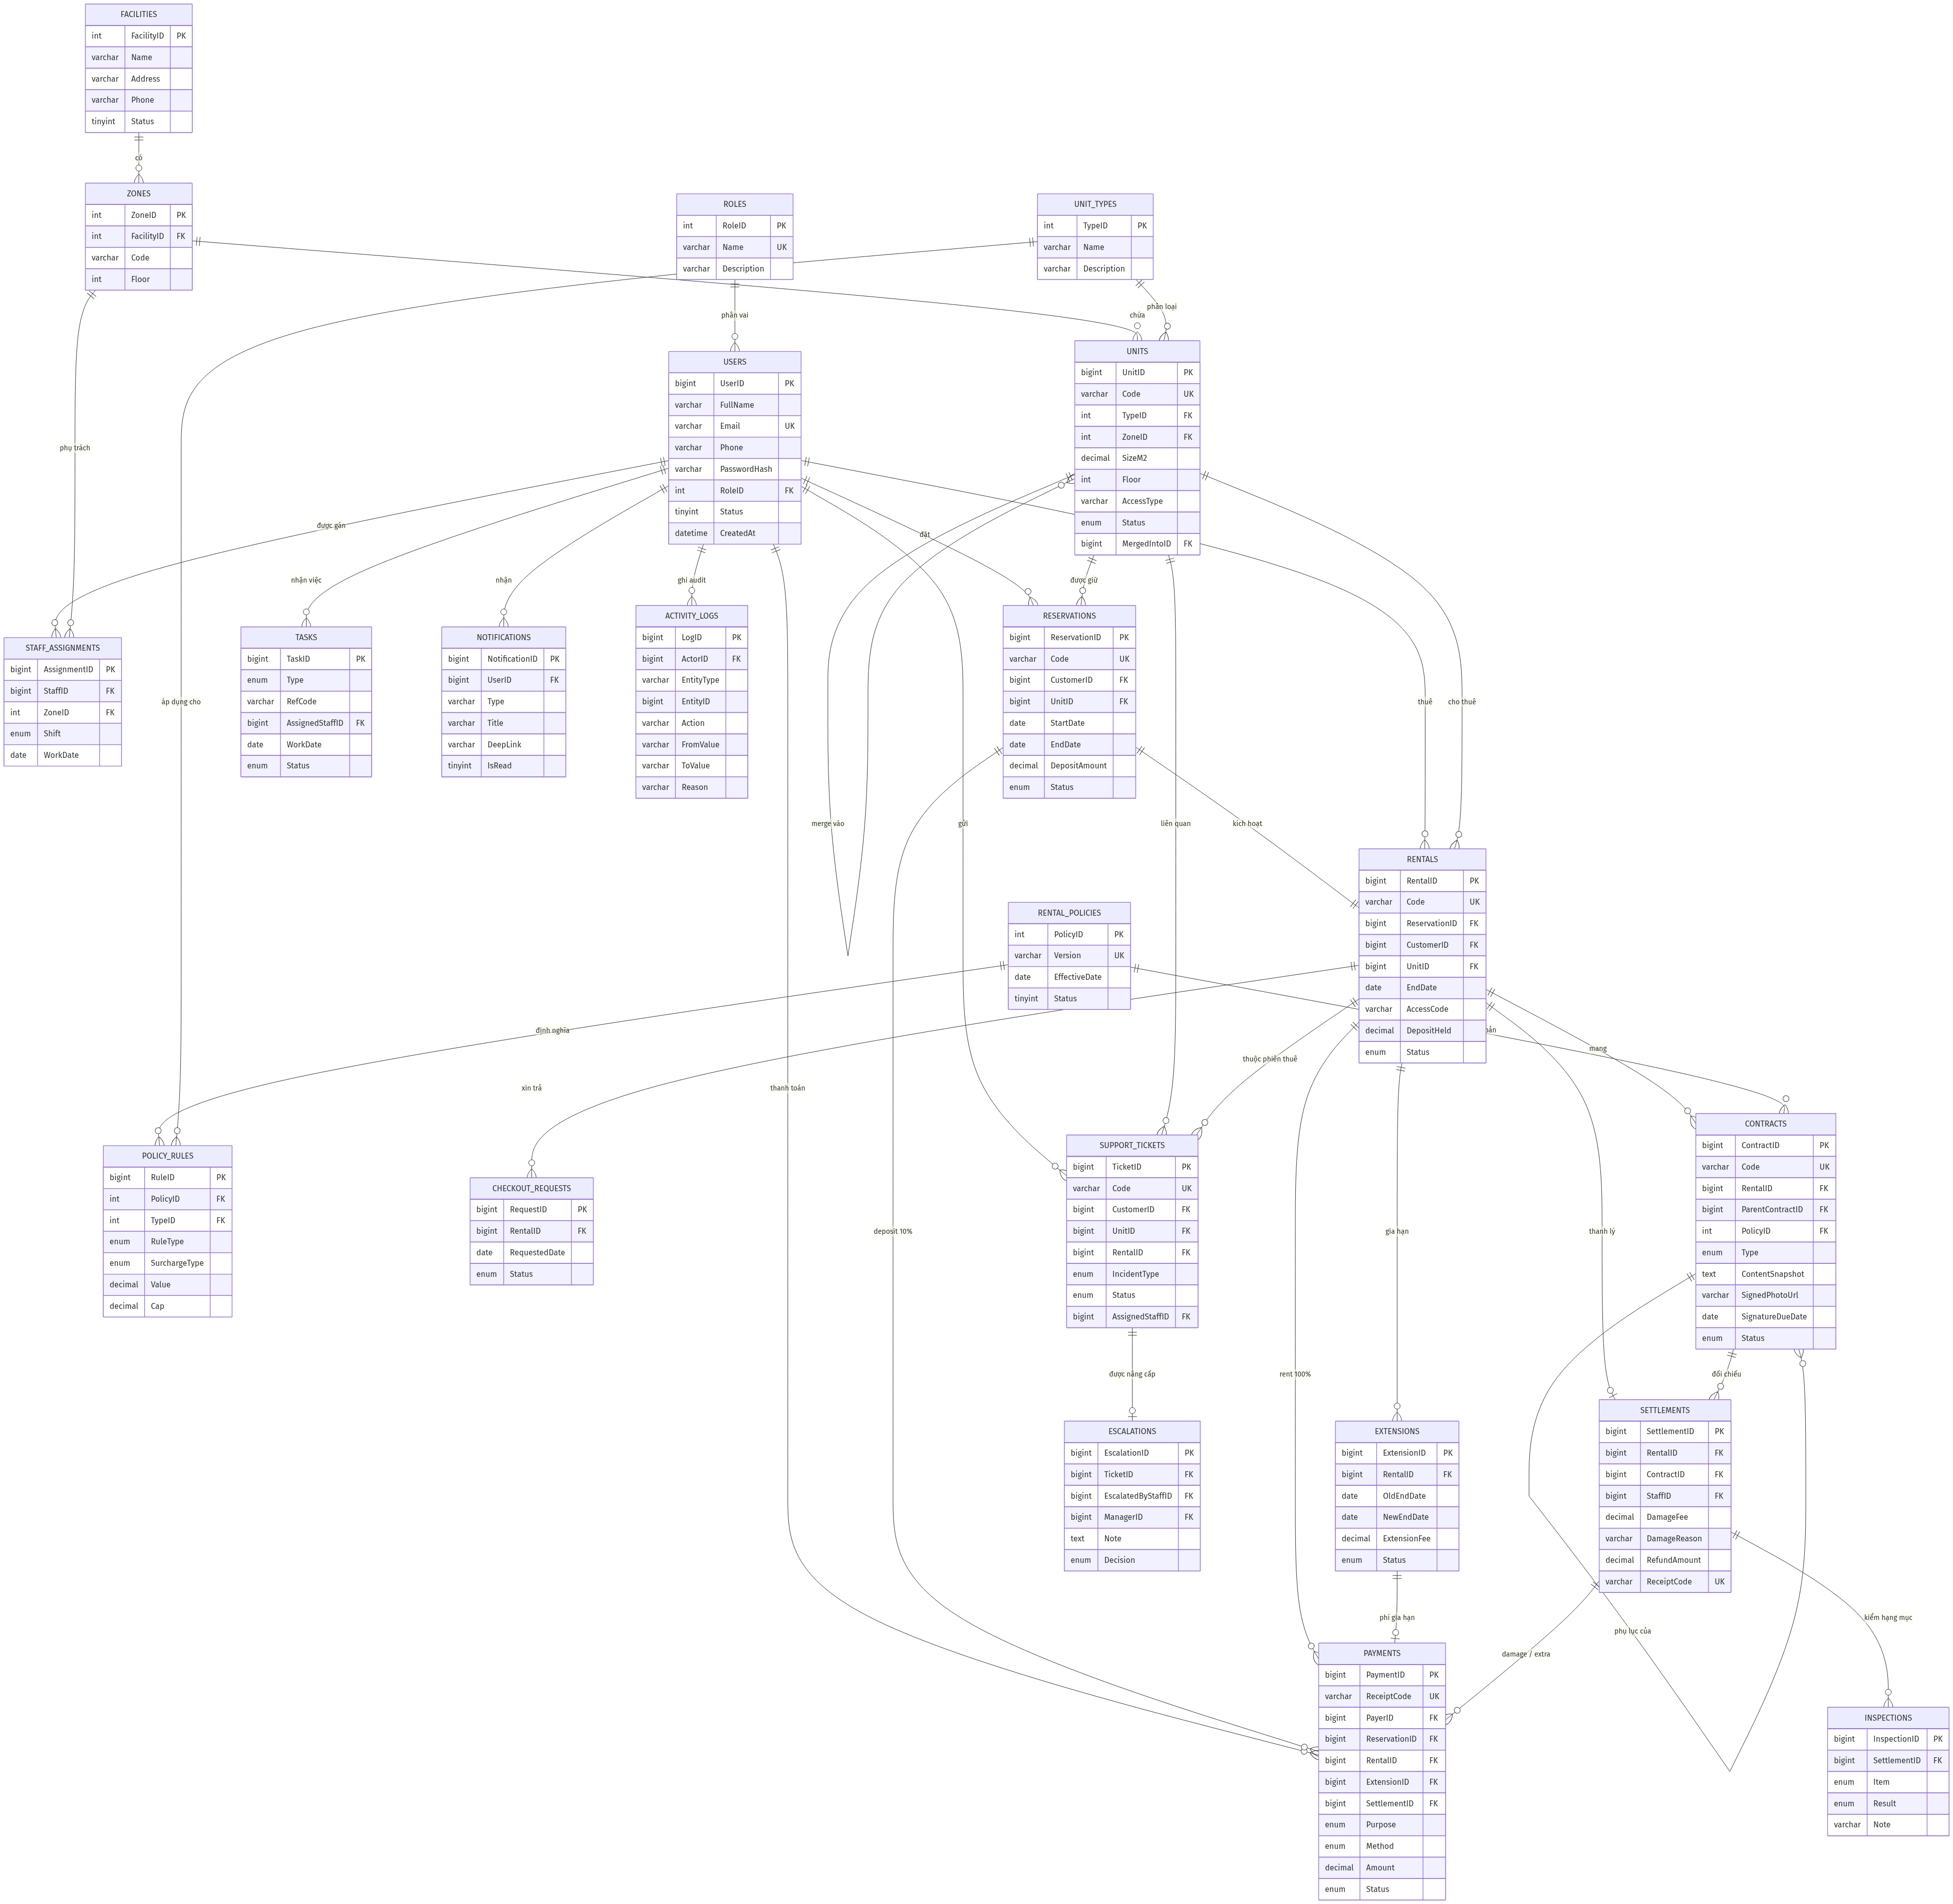
\includegraphics[width=17.5cm]{erd.png}
\caption{ERD toàn hệ thống StorageHub (ký hiệu crow's foot, 22 thực thể / 8 nhóm)}
\label{fig:erd}
\end{figure}
\end{landscape}

%===========================================================
% SECTION 3: STATE CHARTS
%===========================================================
\section{SƠ ĐỒ TRẠNG THÁI (STATE CHART)}

\subsection{Cơ sở lý thuyết và quy ước}

\textbf{Sơ đồ trạng thái (State Chart / State Machine Diagram)} mô tả vòng đời của một đối tượng: các \textbf{trạng thái} nó có thể ở, các \textbf{sự kiện} kích hoạt chuyển trạng thái, \textbf{điều kiện giữ (guard)} viết trong ngoặc vuông $[\ldots]$ phải đúng thì chuyển mới xảy ra, và \textbf{tác dụng phụ} hệ thống thực thi kèm theo. Chấm đặc $\bullet$ là điểm bắt đầu, chấm bao $\circ$ là điểm kết thúc.

Tài liệu này gồm \textbf{7 sơ đồ trạng thái} cho 7 thực thể có vòng đời nghiệp vụ quan trọng nhất: Unit, Reservation, Rental, Contract, Support Ticket, Task, Payment. Trạng thái lưu trong các cột \sqltype{ENUM} đã liệt kê ở Section 2 -- mỗi giá trị enum khớp đúng một trạng thái trên sơ đồ.

\subsection{State chart: Unit (đơn vị lưu trữ)}

Vòng đời phức tạp nhất hệ thống với 6 trạng thái lưu trữ. Unit chỉ về Available khi đã qua Preparing (cleaning xong); nhánh Maintenance phục vụ sửa chữa (từ escalate severe hoặc manager chủ động đặt, kèm lý do); Retired loại unit khỏi tồn kho, có guard chặn khi còn rental/reservation. \textbf{Buffer} ``Available soon'' không phải trạng thái riêng mà là Available + ngày bắt đầu trễ. \textbf{Merge} hai unit liền kề tạo unit mới, unit cũ về Retired.

\begin{xltabular}{\textwidth}{|p{2.6cm}|p{4.4cm}|p{2.6cm}|X|}
\caption{Bảng chuyển dịch trạng thái của Unit} \\
\hline
\textbf{Từ trạng thái} & \textbf{Sự kiện [guard]} & \textbf{Đến} & \textbf{Tác dụng phụ của hệ thống} \\ \hline
\endfirsthead
\hline
\textbf{Từ trạng thái} & \textbf{Sự kiện [guard]} & \textbf{Đến} & \textbf{Tác dụng phụ của hệ thống} \\ \hline
\endhead
$[\bullet]$ & tạo unit mới & Available & Ghi Activity Log \\ \hline
Available & deposit 10\% thành công & Reserved & Sinh reservation BK-; auto-draft hợp đồng CT- \\ \hline
Reserved & check-in hoàn tất [hợp đồng đã ký] & Rented & Sinh rental RT-; cấp access code \\ \hline
Reserved & hết hạn giữ chỗ / huỷ đặt & Available & Hoàn cọc theo policy; Activity Log \\ \hline
Rented & checkout + settlement hoàn tất & Preparing & Sinh task cleaning TL- \\ \hline
Preparing & cleaning task xong & Available & Đơn giản nhất -- sẵn sàng cho khách mới \\ \hline
Preparing & cleaning xong [có reservation kế tiếp] & Reserved & Trực tiếp sang giữ chỗ kế tiếp \\ \hline
Rented & escalate mức severe & Maintenance & Sinh escalation; tái định vị khách \\ \hline
Available & manager đặt [bắt buộc reason] & Maintenance & Activity Log kèm lý do \\ \hline
Maintenance & sửa chữa xong & Preparing & Sinh task cleaning trước khi cho thuê lại \\ \hline
Maintenance & bỏ khỏi tồn kho & Retired & Activity Log \\ \hline
Available & retire [guard: không rental/reservation] & Retired & Chặn thao tác nếu còn lịch \\ \hline
Reserved & retire [guard: không rental/reservation] & Retired & Chặn thao tác nếu còn lịch \\ \hline
Rented/Available & merge 2 unit liền kề [guard: cả hai phía rỗng lịch] & Retired $\rightarrow$ unit mới & Unit cũ trỏ \attr{MergedIntoID} \\ \hline
\end{xltabular}

\begin{figure}[H]
\centering
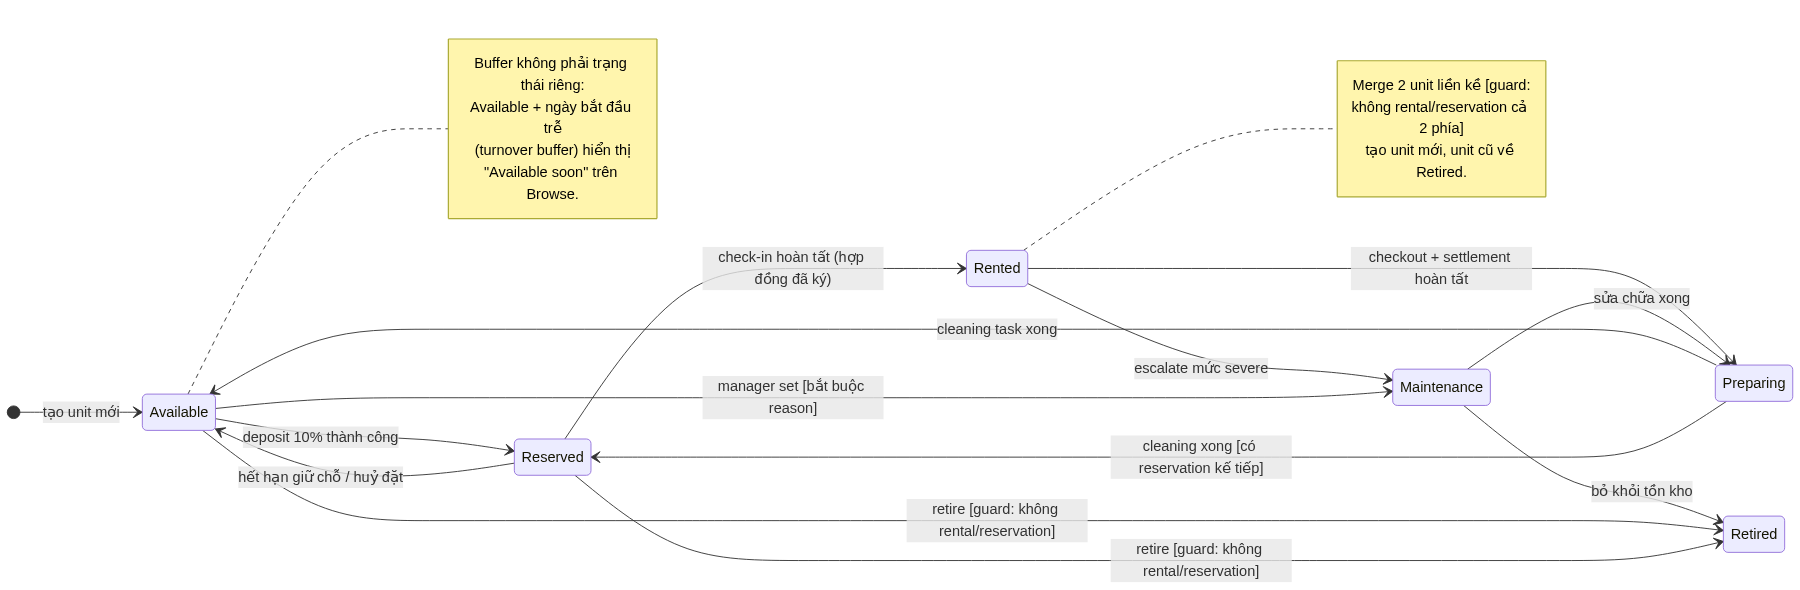
\includegraphics[width=\textwidth]{state-unit.png}
\caption{State chart Unit}
\label{fig:state-unit}
\end{figure}

\subsection{State chart: Reservation (đặt chỗ -- BK-)}

Khách duyệt unit trên Browse rồi xác nhận Booking Summary: reservation sinh ra ở PendingPayment và chỉ thực sự giữ unit khi cổng thanh toán xác nhận cọc 10\%. Thanh toán thất bại được retry ngay tại chỗ; bỏ modal thì không giữ unit. Sau khi Reserved, có ba lối ra: check-in (trả 100\% + ký hợp đồng, sinh Rental), quá hạn check-in (unit trả về Available), hoặc khách chủ động huỷ (hoàn cọc theo policy).

\begin{xltabular}{\textwidth}{|p{2.6cm}|p{4.4cm}|p{2.6cm}|X|}
\caption{Bảng chuyển dịch trạng thái của Reservation} \\
\hline
\textbf{Từ trạng thái} & \textbf{Sự kiện [guard]} & \textbf{Đến} & \textbf{Tác dụng phụ của hệ thống} \\ \hline
\endfirsthead
\hline
\textbf{Từ trạng thái} & \textbf{Sự kiện [guard]} & \textbf{Đến} & \textbf{Tác dụng phụ của hệ thống} \\ \hline
\endhead
$[\bullet]$ & khách đặt unit (Booking Summary) & PendingPayment & Mở Payment Modal; đơn vị vẫn hiển thị Available \\ \hline
PendingPayment & gateway xác nhận deposit & Reserved & Unit $\rightarrow$ Reserved; auto-draft hợp đồng CT- \\ \hline
PendingPayment & payment fail [retry / đổi method] & PendingPayment & ``No money was taken''; sau 2 lần gợi ý đổi method \\ \hline
PendingPayment & khách bỏ qua & $[\circ]$ & Không giữ unit \\ \hline
Reserved & trả 100\% rent + ký hợp đồng & CheckedIn & Sinh rental RT-; cấp access code; hợp đồng Active \\ \hline
Reserved & quá hạn check-in & Expired & Unit trả về Available; Activity Log \\ \hline
Reserved & huỷ đặt & Cancelled & Hoàn cọc theo policy; Activity Log \\ \hline
\end{xltabular}

\begin{figure}[H]
\centering
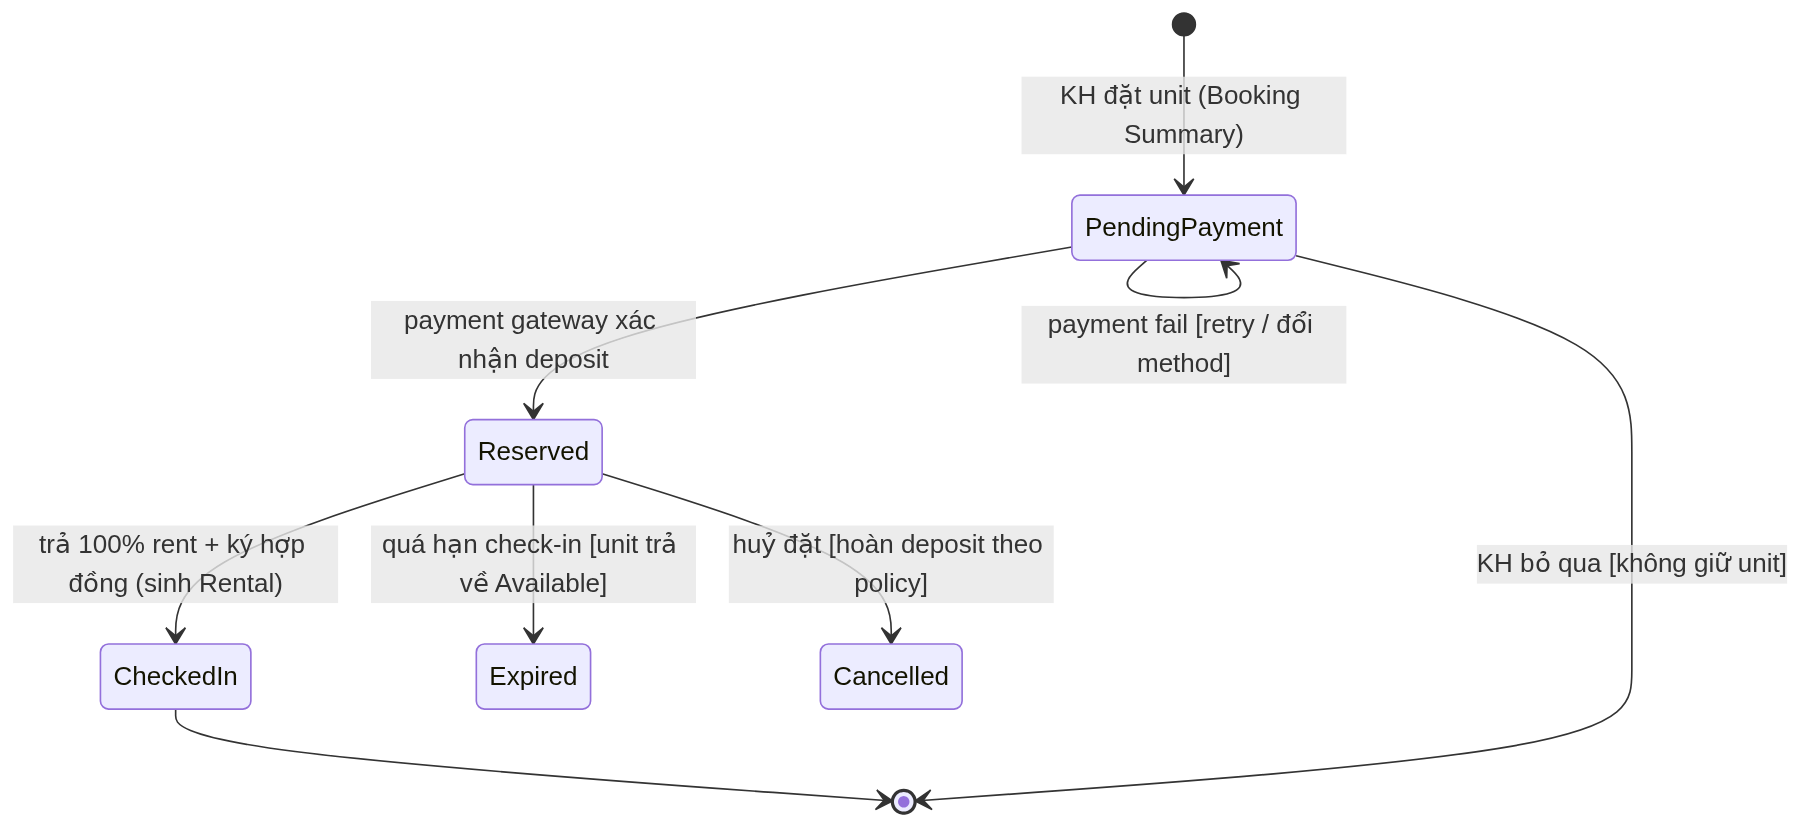
\includegraphics[width=\textwidth]{state-reservation.png}
\caption{State chart Reservation}
\label{fig:state-reservation}
\end{figure}

\subsection{State chart: Rental (phiên thuê -- RT-)}

Rental sinh ra khi check-in xong và mang access code. Điểm thiết kế quan trọng nhất: \textbf{gia hạn hiệu lực theo thanh toán} -- \attr{EndDate} của rental dịch ngay khi phí gia hạn được xác nhận, phụ lục hợp đồng chỉ là hồ sơ giấy đi sau, không giữ unit. Guard chống xung đột lịch: ngày trả mới nhất luôn thắng (``Latest new checkout'') để không đè reservation kế tiếp. Kết thúc phiên thuê phải qua CheckoutRequested + settlement.

\begin{xltabular}{\textwidth}{|p{2.6cm}|p{4.4cm}|p{2.6cm}|X|}
\caption{Bảng chuyển dịch trạng thái của Rental} \\
\hline
\textbf{Từ trạng thái} & \textbf{Sự kiện [guard]} & \textbf{Đến} & \textbf{Tác dụng phụ của hệ thống} \\ \hline
\endfirsthead
\hline
\textbf{Từ trạng thái} & \textbf{Sự kiện [guard]} & \textbf{Đến} & \textbf{Tác dụng phụ của hệ thống} \\ \hline
\endhead
$[\bullet]$ & check-in xong & Active & Cấp access code \\ \hline
Active & gia hạn [phí đã trả] & Active & \attr{EndDate} dịch ngay; sinh extension + addendum chờ ký \\ \hline
Active & khách gửi checkout request & CheckoutRequested & Sinh task checkout TL- \\ \hline
CheckoutRequested & settlement hoàn tất & Closed & Hoàn = cọc $-$ phí hư hại; unit $\rightarrow$ Preparing \\ \hline
Closed & -- & $[\circ]$ & Kết thúc phiên thuê \\ \hline
\end{xltabular}

\begin{figure}[H]
\centering
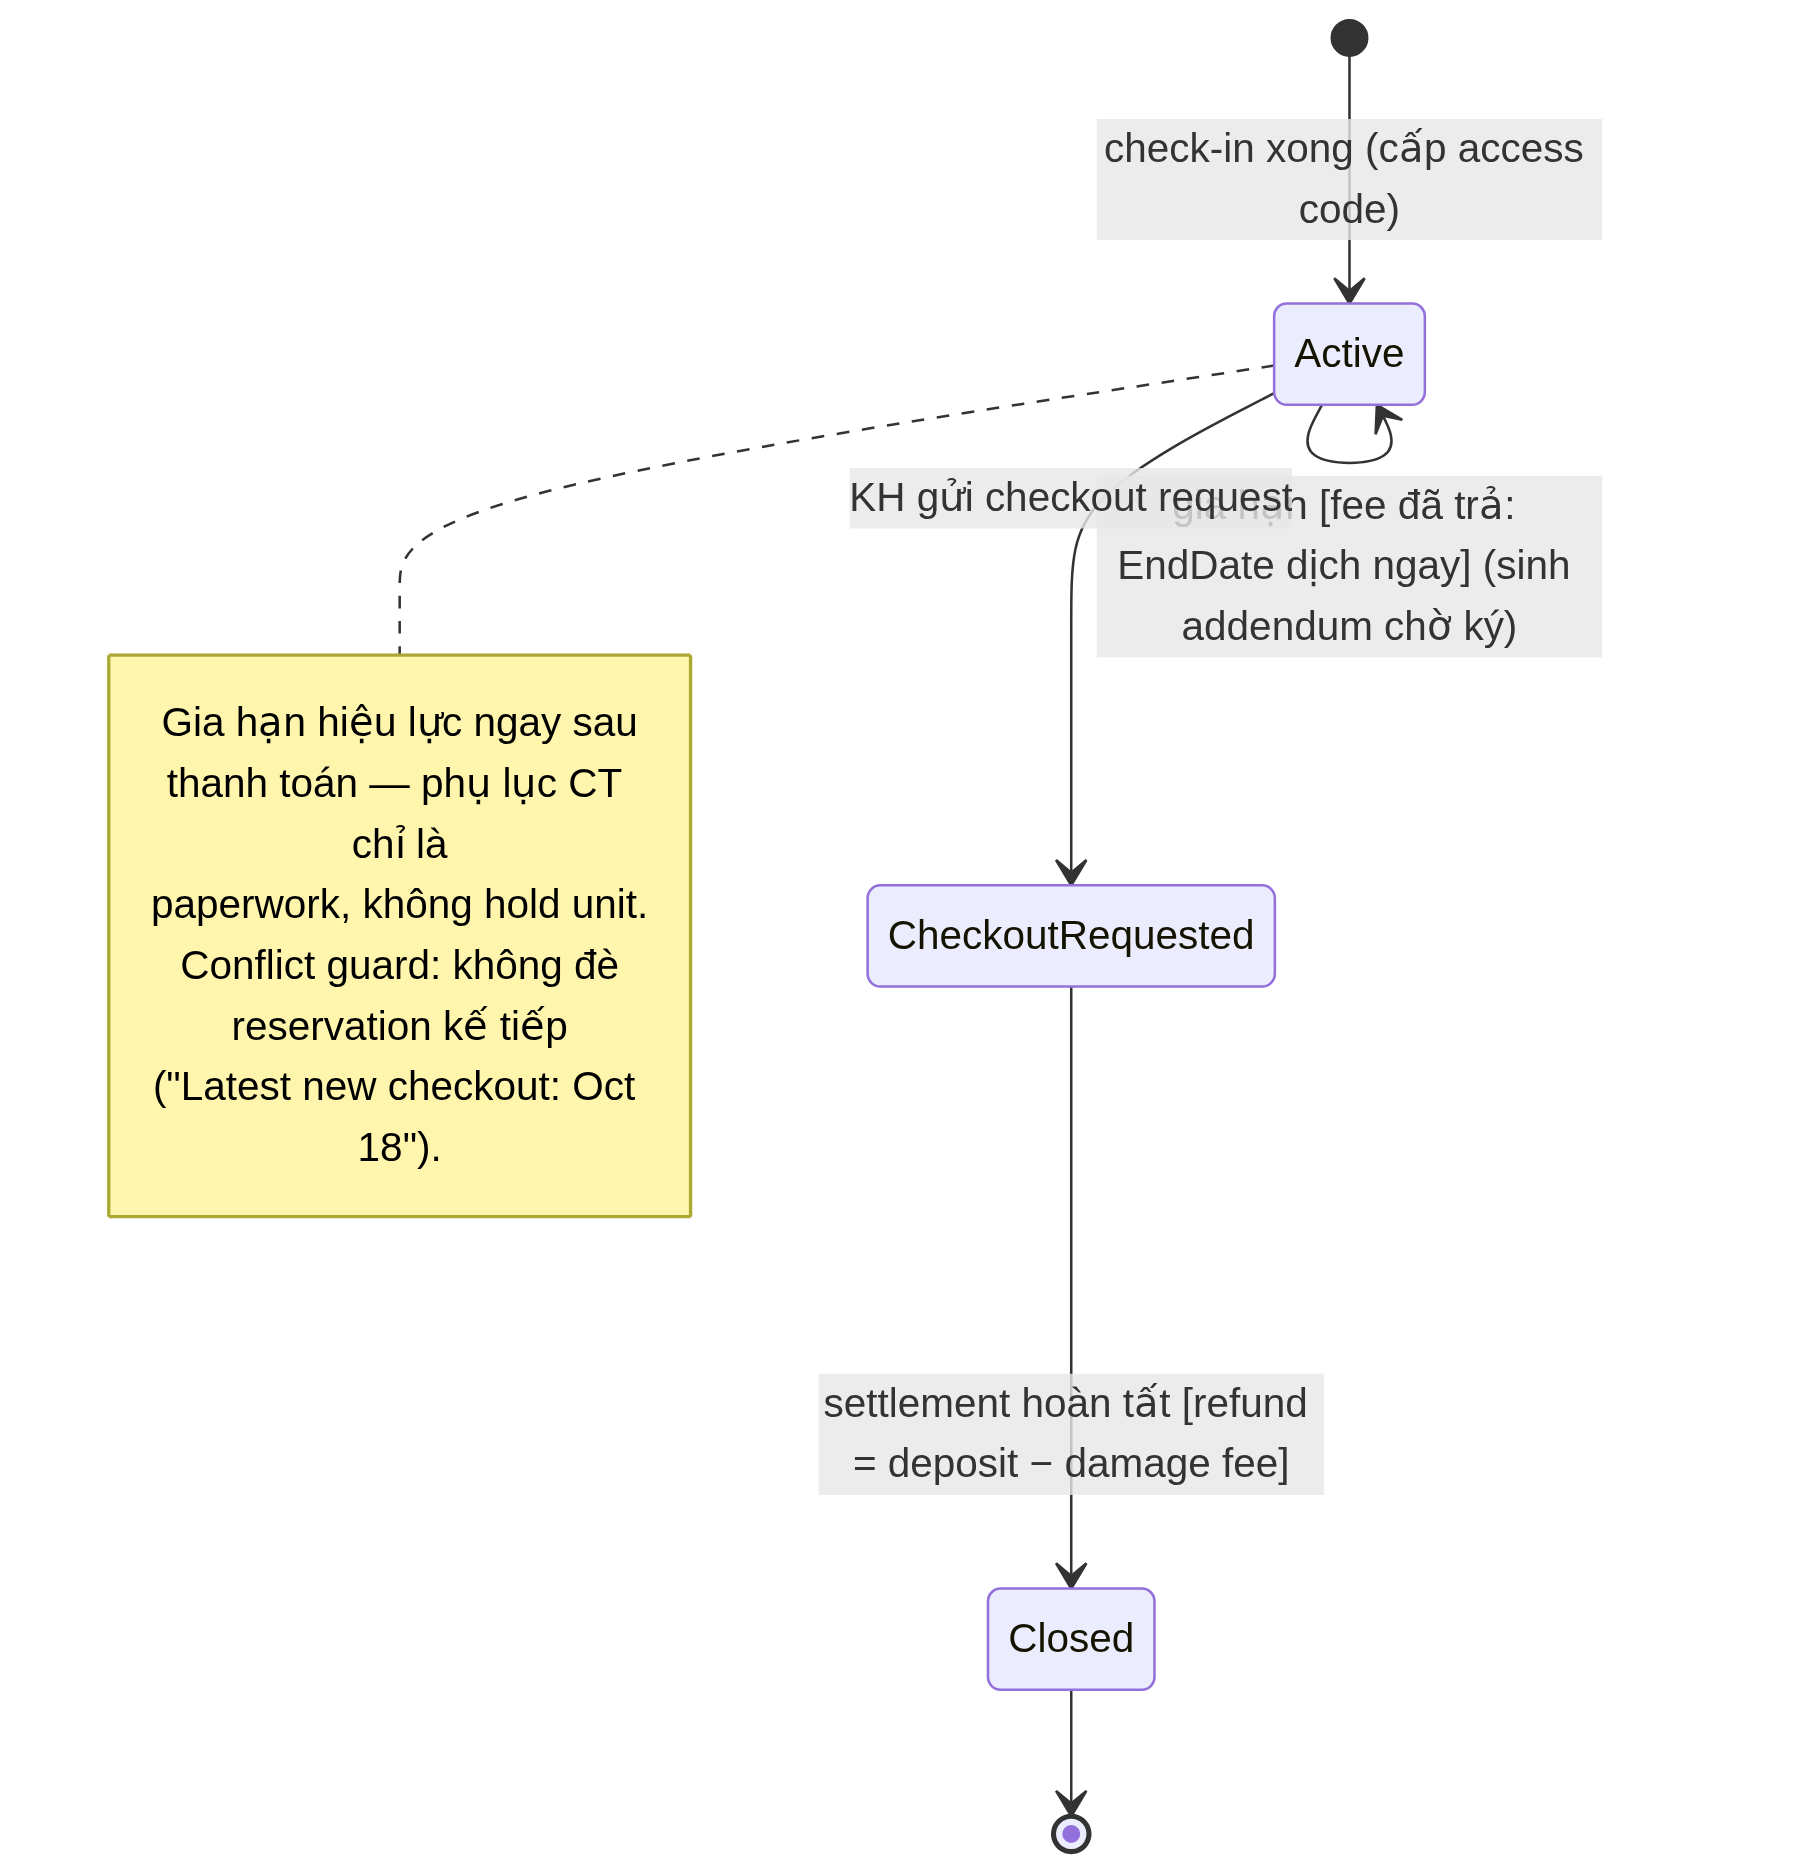
\includegraphics[width=\textwidth]{state-rental.png}
\caption{State chart Rental}
\label{fig:state-rental}
\end{figure}

\subsection{State chart: Contract (hợp đồng -- CT-)}

Hợp đồng gốc: auto-draft ngay khi đặt cọc thành công (khoá phiên bản policy), staff in tại quầy, khách ký + staff chụp ảnh attach, rental kích hoạt thì hợp đồng Active; settlement đối chiếu số hợp đồng khi đóng. \textbf{Hợp đồng không ai sửa được} -- muốn sửa phải draft lại; vì thế gia hạn đi theo nhánh \textbf{phụ lục (addendum)}: auto-draft sau khi trả phí, chờ ký với hạn 7 ngày (quá hạn hiển thị banner amber + nhắc việc), ký xong hợp đồng gốc bị Superseded về ngày kết thúc.

\begin{xltabular}{\textwidth}{|p{2.6cm}|p{4.4cm}|p{2.6cm}|X|}
\caption{Bảng chuyển dịch trạng thái của Contract} \\
\hline
\textbf{Từ trạng thái} & \textbf{Sự kiện [guard]} & \textbf{Đến} & \textbf{Tác dụng phụ của hệ thống} \\ \hline
\endfirsthead
\hline
\textbf{Từ trạng thái} & \textbf{Sự kiện [guard]} & \textbf{Đến} & \textbf{Tác dụng phụ của hệ thống} \\ \hline
\endhead
$[\bullet]$ & deposit thành công & Draft & Auto-draft; snapshot theo phiên bản policy \\ \hline
Draft & staff in tại quầy & Printed & Chờ ảnh bản ký \\ \hline
Printed & khách ký + staff chụp ảnh attach & Signed & Lưu \attr{SignedPhotoUrl} \\ \hline
Signed & rental kích hoạt & Active & Hợp đồng gốc có hiệu lực \\ \hline
Active & settlement đối chiếu số hợp đồng & Closed & Kết thúc cùng phiên thuê \\ \hline
Active & addendum thay ngày kết thúc & Superseded & Hợp đồng gốc nhường cho phụ lục \\ \hline
Draft & addendum gia hạn [phí đã trả] & AwaitingSignature & Auto-draft phụ lục; \attr{ParentContractID} trỏ gốc \\ \hline
AwaitingSignature & ký tại quầy [hạn 7 ngày] & Signed & Bell reminder trước hạn \\ \hline
AwaitingSignature & quá hạn & AwaitingSignature & Banner amber + nhắc việc (tự vòng) \\ \hline
\end{xltabular}

\begin{figure}[H]
\centering
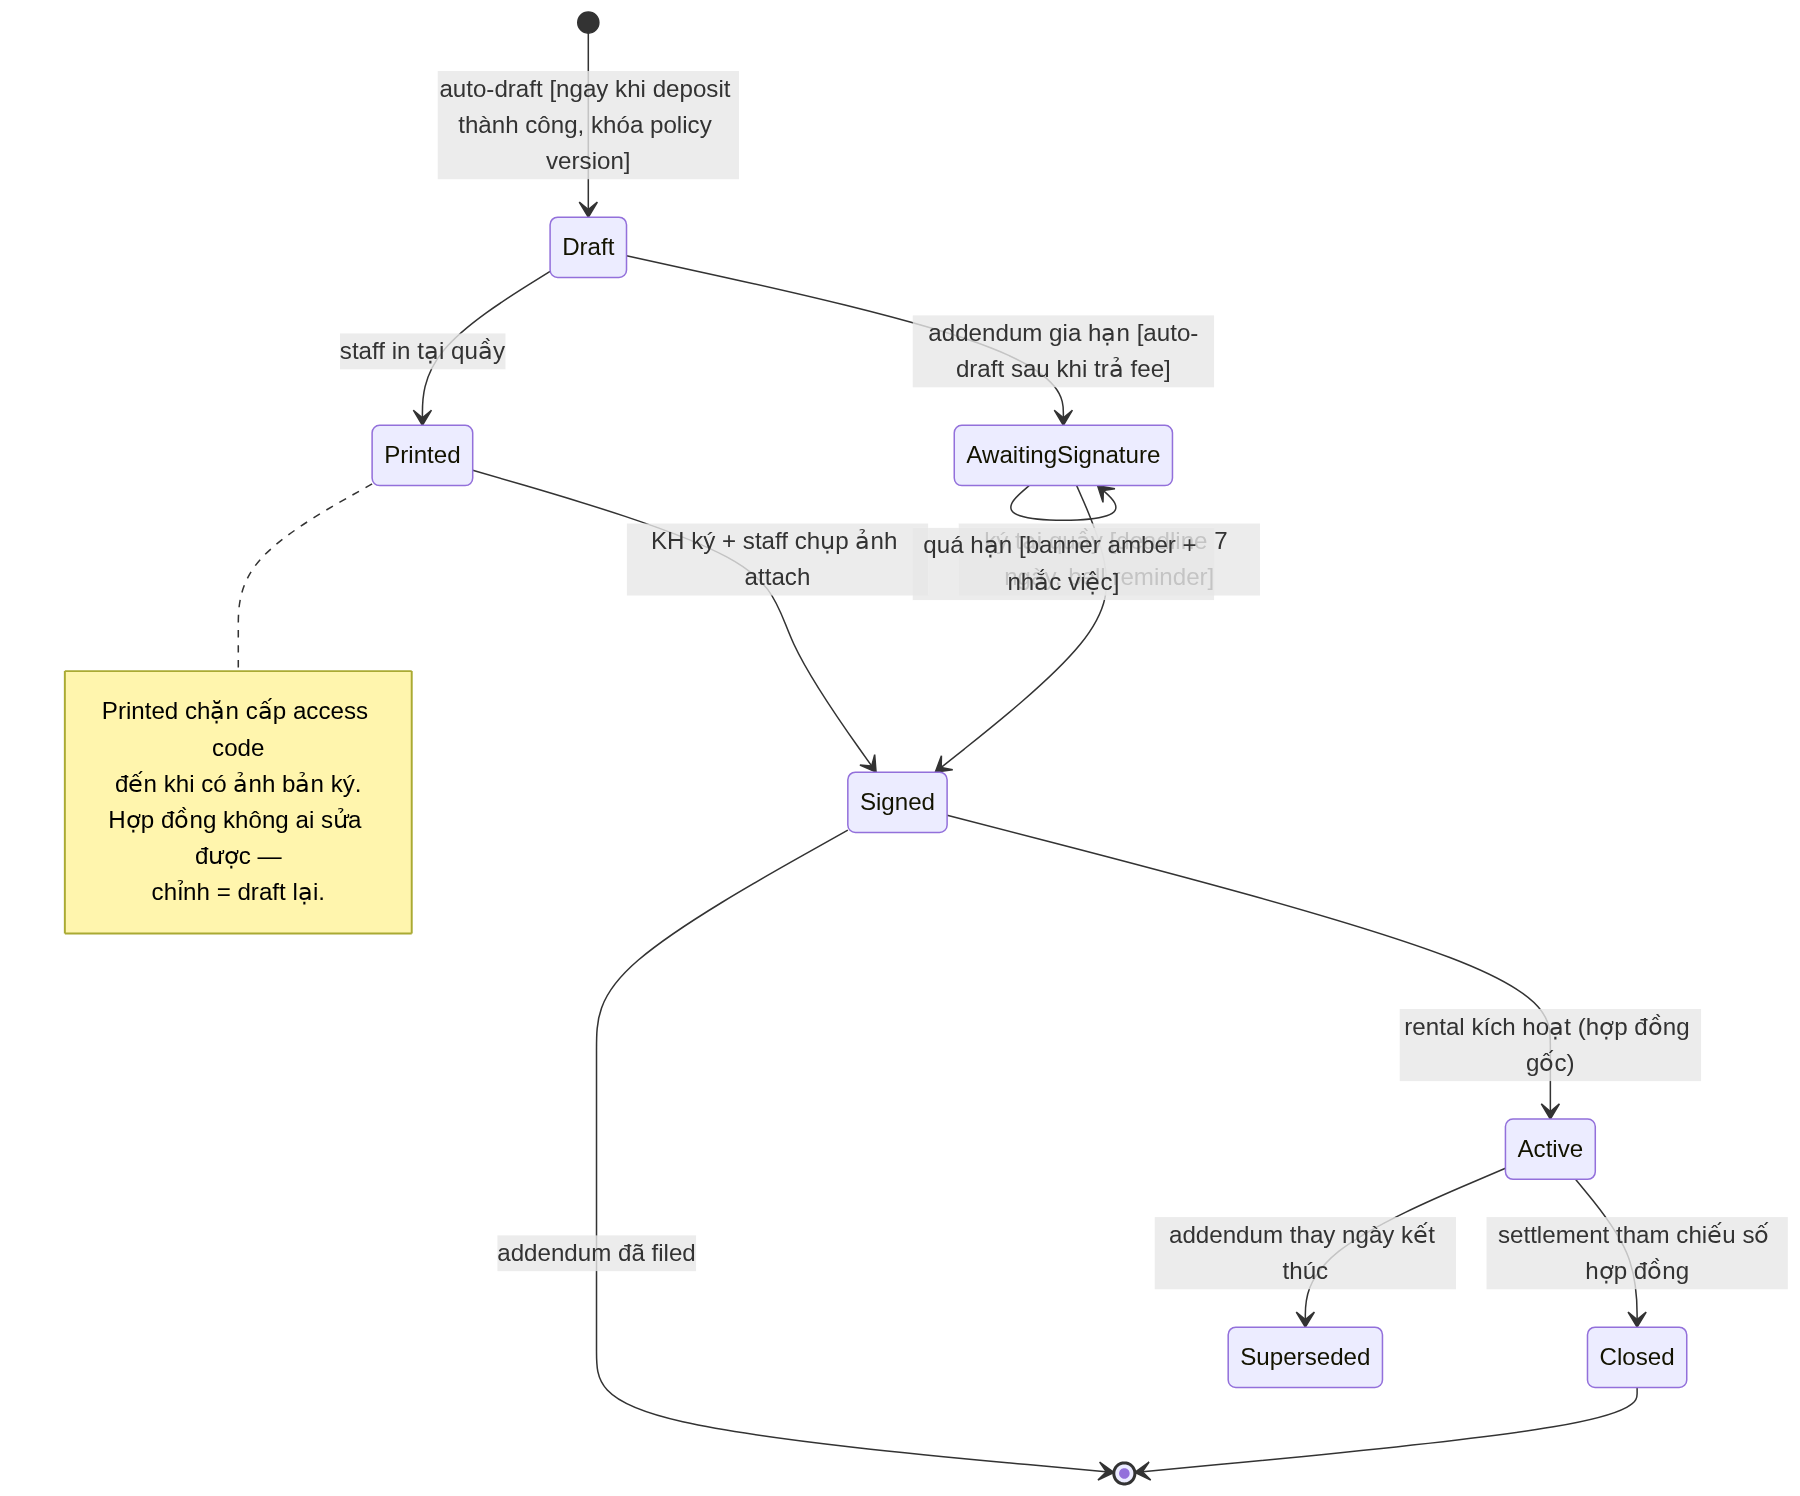
\includegraphics[width=\textwidth]{state-contract.png}
\caption{State chart Contract}
\label{fig:state-contract}
\end{figure}

\subsection{State chart: Support Ticket (hỗ trợ -- SR-)}

Ticket vào Open khi khách gửi support request, được định tuyến tới staff trực ca theo unit + shift. Staff xử lý xong thì Resolved (kèm note); nếu vượt thẩm quyền thì Escalated -- \textbf{bắt buộc có note}. Manager có hai lối: quyết định severe (unit $\rightarrow$ Maintenance + tái định vị khách) hoặc trả về staff kèm guidance. Ticket severe không bao giờ bị bỏ rơi: quyết định ghi Activity Log, khách nhận notification từng bước.

\begin{xltabular}{\textwidth}{|p{2.6cm}|p{4.4cm}|p{2.6cm}|X|}
\caption{Bảng chuyển dịch trạng thái của Support Ticket} \\
\hline
\textbf{Từ trạng thái} & \textbf{Sự kiện [guard]} & \textbf{Đến} & \textbf{Tác dụng phụ của hệ thống} \\ \hline
\endfirsthead
\hline
\textbf{Từ trạng thái} & \textbf{Sự kiện [guard]} & \textbf{Đến} & \textbf{Tác dụng phụ của hệ thống} \\ \hline
\endhead
$[\bullet]$ & khách gửi support request & Open & Định tuyến theo unit + shift \\ \hline
Open & route tới staff trực ca & InProgress & Gán \attr{AssignedStaffID}; sinh task support TL- \\ \hline
InProgress & staff xử lý xong + note & Resolved & Thông báo cho khách \\ \hline
InProgress & staff escalate [bắt buộc note] & Escalated & Sinh escalation; manager nhận notification \\ \hline
Escalated & manager đánh giá severe & Resolved & Unit $\rightarrow$ Maintenance; tái định vị khách; Activity Log \\ \hline
Escalated & manager trả về staff [kèm guidance] & InProgress & Staff tiếp tục theo hướng dẫn \\ \hline
\end{xltabular}

\begin{figure}[H]
\centering
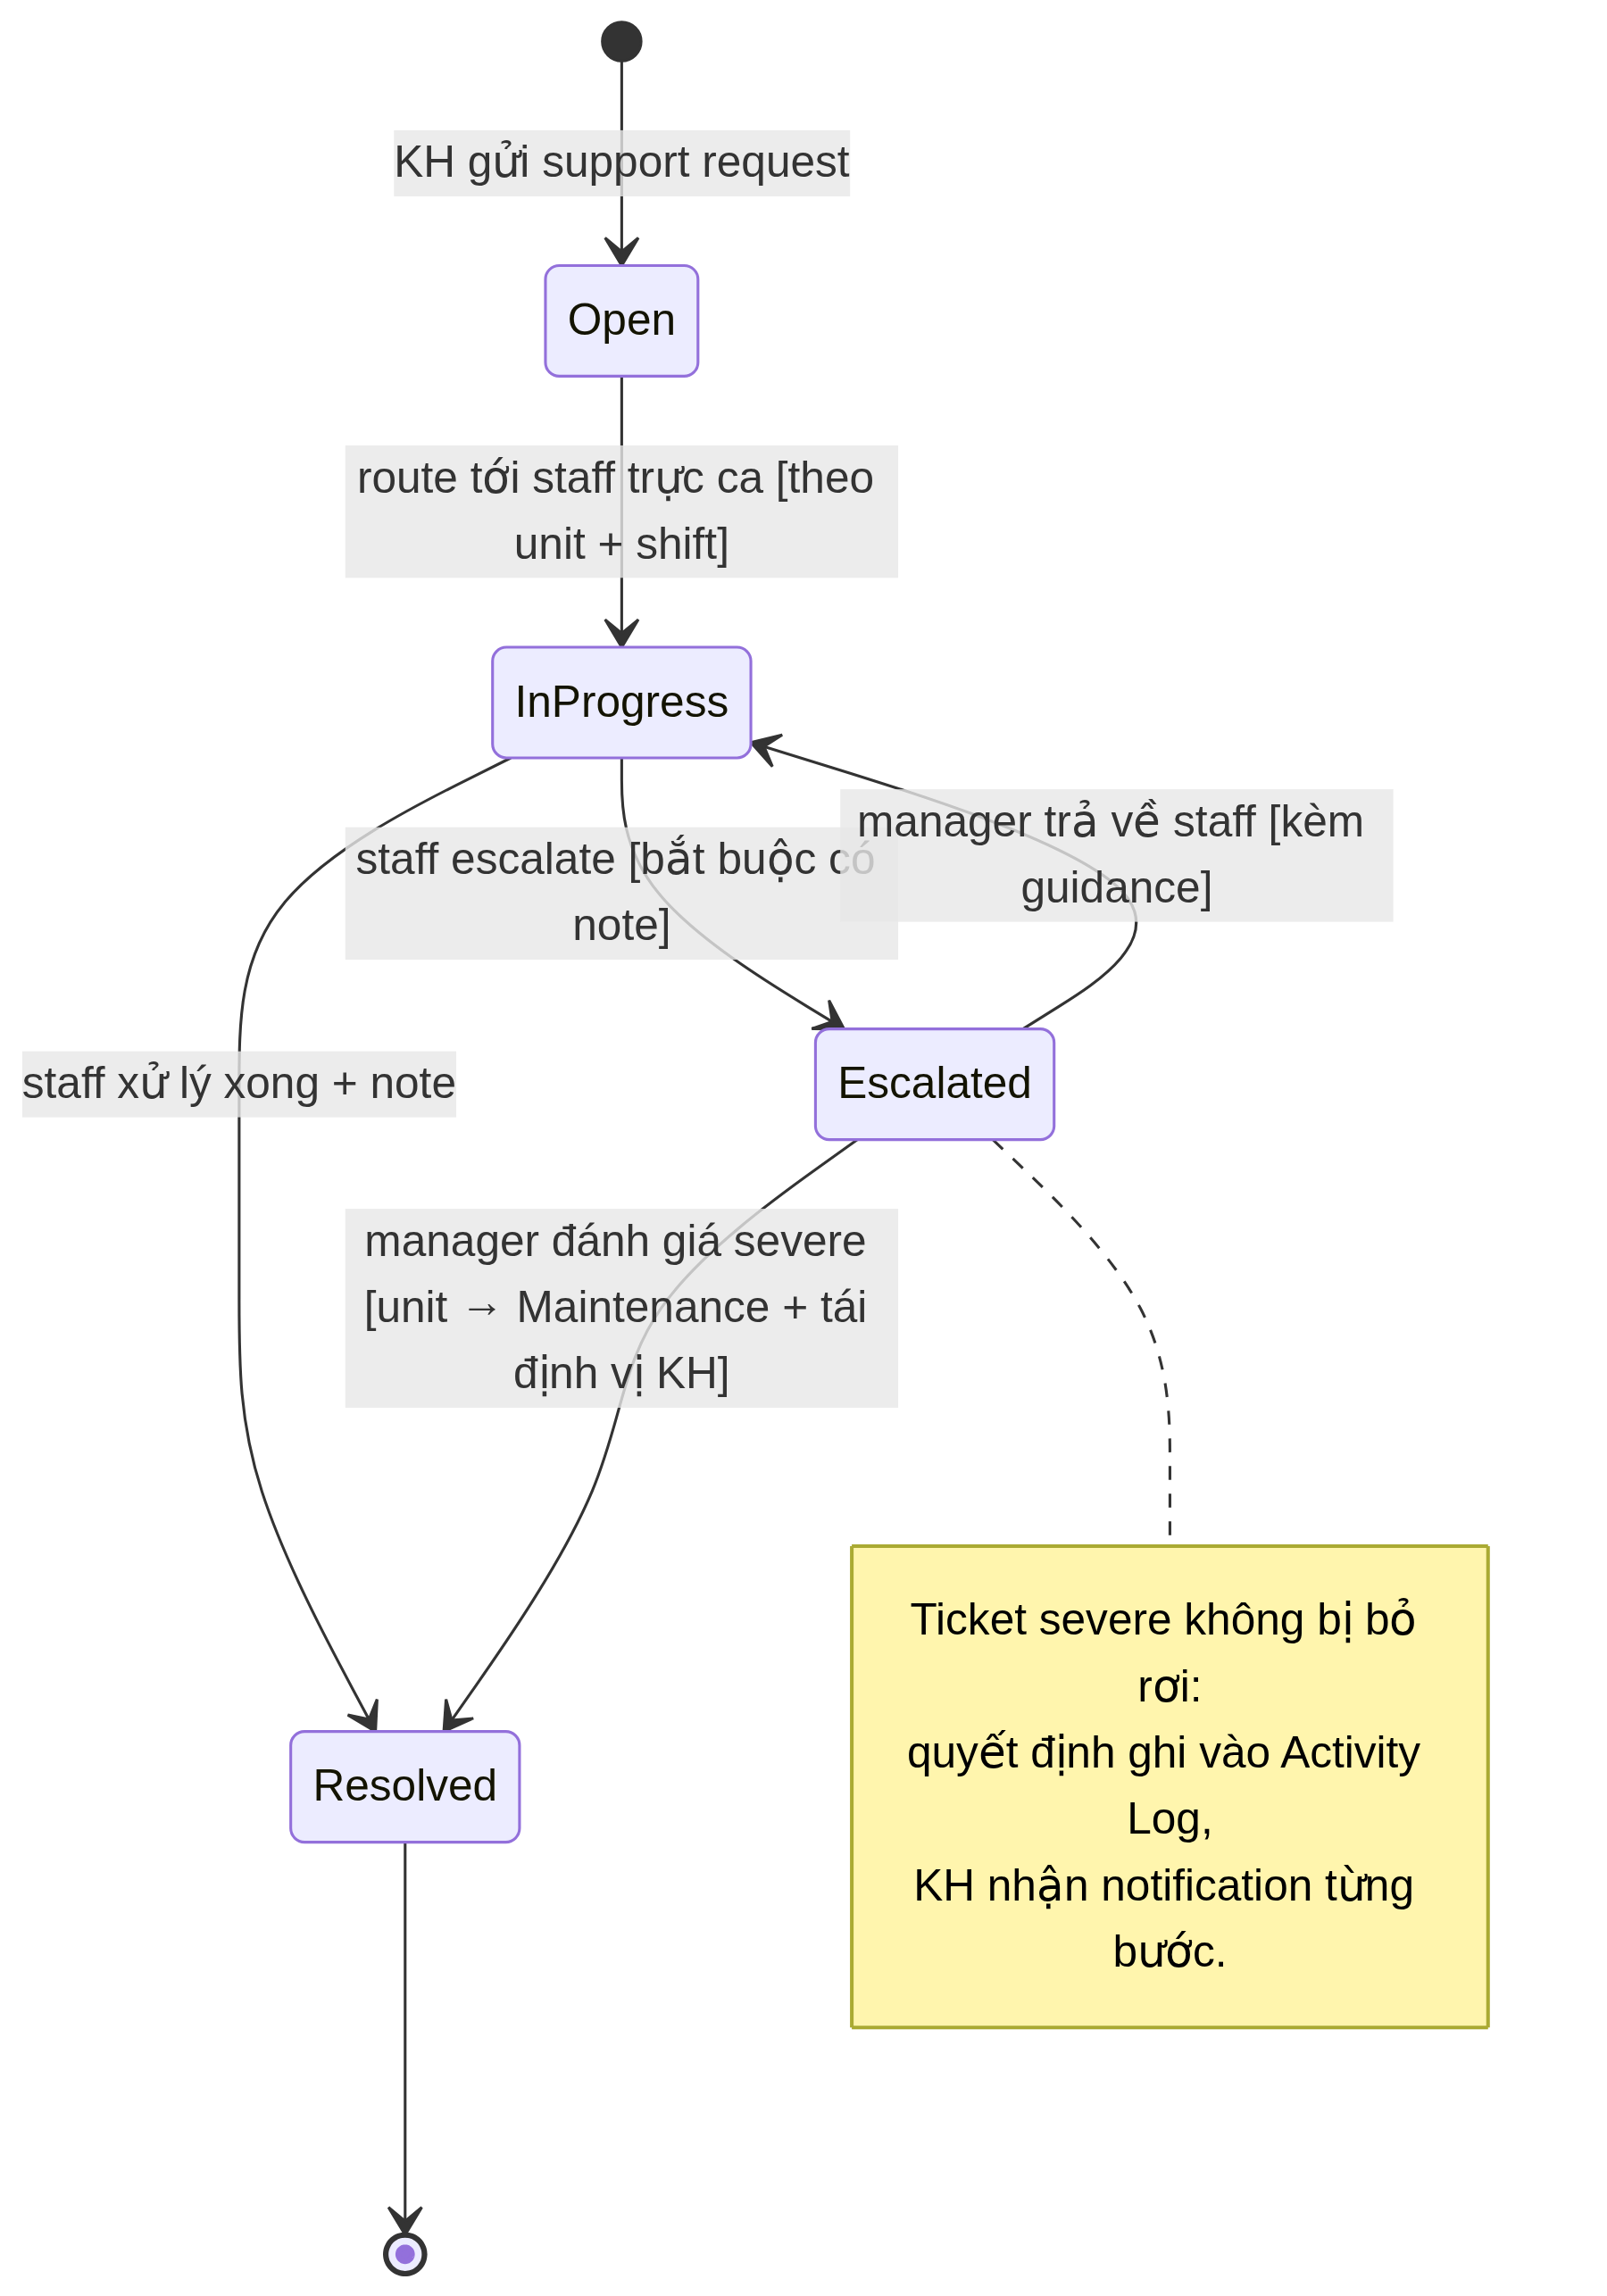
\includegraphics[width=0.82\textwidth]{state-ticket.png}
\caption{State chart Support Ticket}
\label{fig:state-ticket}
\end{figure}

\subsection{State chart: Task (kanban)}

Task sinh tự động từ nghiệp vụ (check-in, checkout, cleaning, support, contract) và được staff thao tác trên bảng kanban. Guard trung tâm: chỉ được kéo sang Done khi \textbf{bước chốt} đã hoàn tất -- task check-in cần payment, task checkout cần settlement, task contract cần ảnh bản ký. Kéo sai thì state ``snap-back'' về InProgress kèm toast chỉ đúng tên bước còn thiếu.

\begin{xltabular}{\textwidth}{|p{2.6cm}|p{4.4cm}|p{2.6cm}|X|}
\caption{Bảng chuyển dịch trạng thái của Task} \\
\hline
\textbf{Từ trạng thái} & \textbf{Sự kiện [guard]} & \textbf{Đến} & \textbf{Tác dụng phụ của hệ thống} \\ \hline
\endfirsthead
\hline
\textbf{Từ trạng thái} & \textbf{Sự kiện [guard]} & \textbf{Đến} & \textbf{Tác dụng phụ của hệ thống} \\ \hline
\endhead
$[\bullet]$ & hệ thống sinh task [check-in / checkout / cleaning / support / contract] & ToDo & Xuất hiện trên kanban của staff trực ca \\ \hline
ToDo & staff kéo thả hoặc mở task & InProgress & -- \\ \hline
InProgress & hoàn tất bước chốt [guard: payment / settlement / ảnh bản ký] & Done & Cập nhật hồ sơ liên quan \\ \hline
Done & snap-back [thiếu bước chốt] & InProgress & Toast chỉ tên bước thiếu \\ \hline
\end{xltabular}

\begin{figure}[H]
\centering
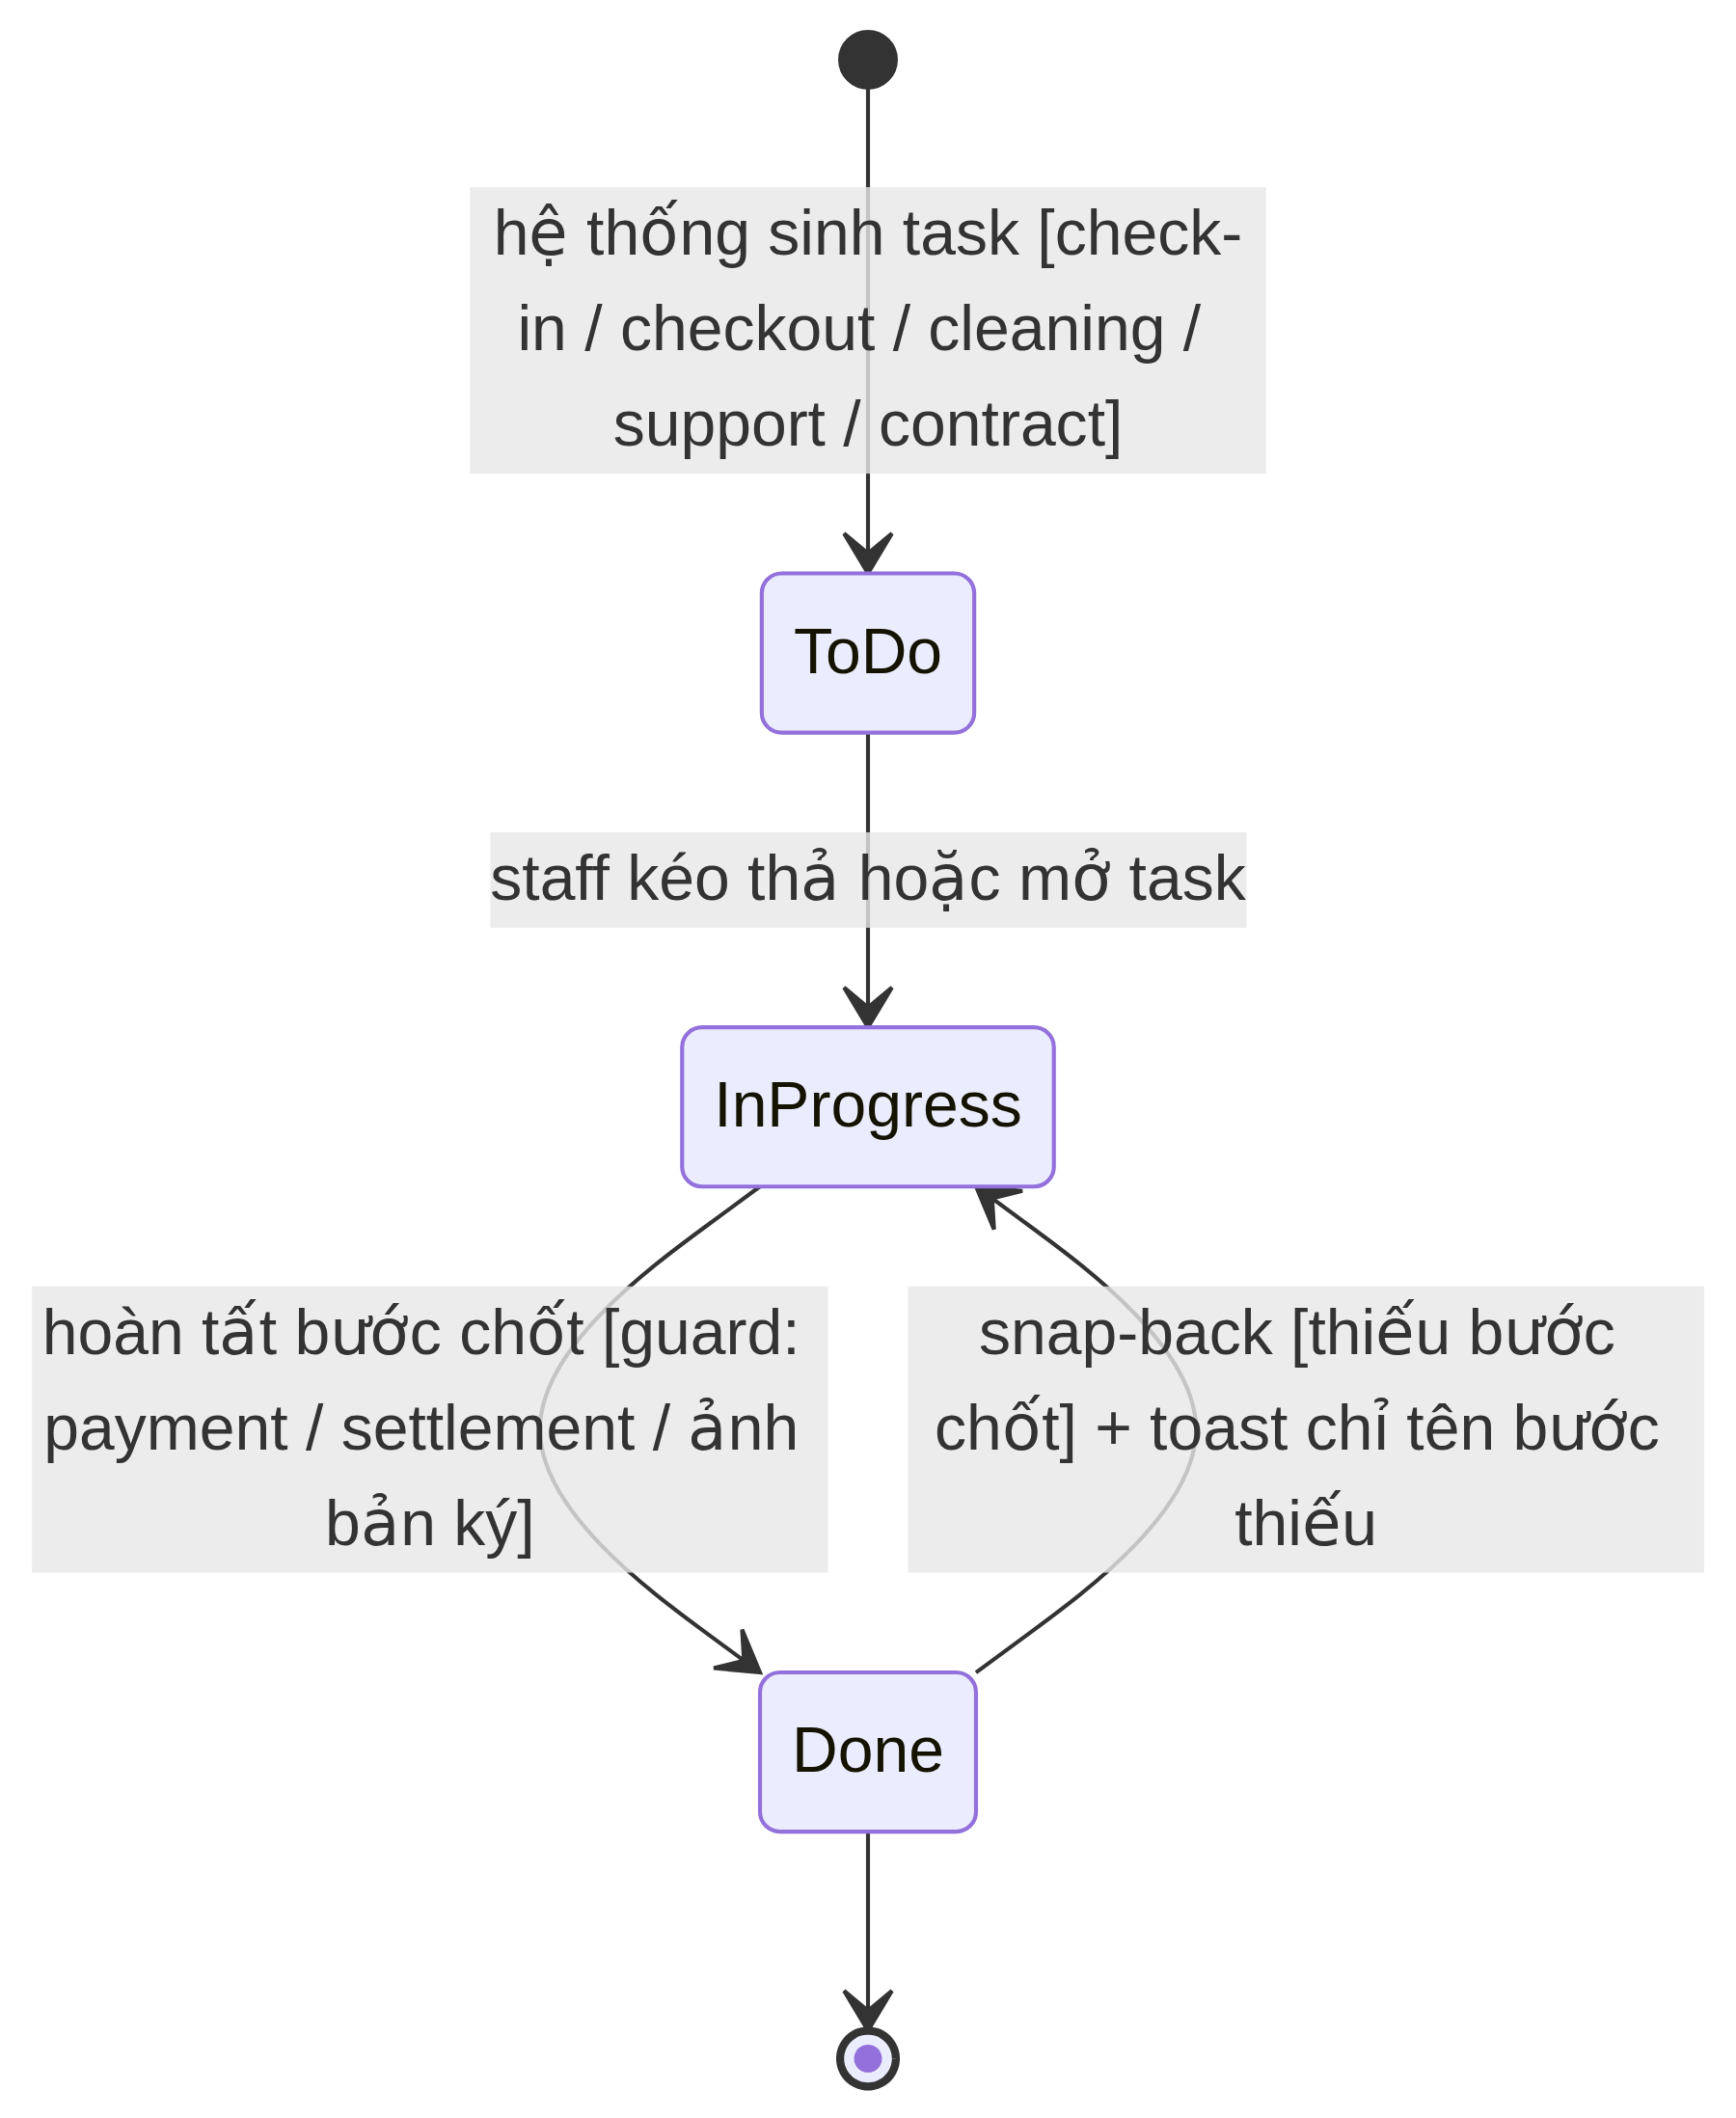
\includegraphics[width=0.88\textwidth]{state-task.png}
\caption{State chart Task}
\label{fig:state-task}
\end{figure}

\subsection{State chart: Payment (cổng thanh toán mô phỏng)}

Cả 3 touchpoint tiền (cọc 10\%, thuê 100\%, phí gia hạn) dùng chung một máy trạng thái của Payment Modal. Bấm Pay khóa nút back, spinner 1.5--2s; gateway mô phỏng trả Succeeded hoặc Failed (``No money was taken''); QR hết hạn sau khoảng 5 phút thì về Expired và khách chọn lại method. Chỉ Succeeded mới đổi trạng thái nghiệp vụ (reservation/rental/extension) và bắn toast + bell.

\begin{xltabular}{\textwidth}{|p{2.6cm}|p{4.4cm}|p{2.6cm}|X|}
\caption{Bảng chuyển dịch trạng thái của Payment} \\
\hline
\textbf{Từ trạng thái} & \textbf{Sự kiện [guard]} & \textbf{Đến} & \textbf{Tác dụng phụ của hệ thống} \\ \hline
\endfirsthead
\hline
\textbf{Từ trạng thái} & \textbf{Sự kiện [guard]} & \textbf{Đến} & \textbf{Tác dụng phụ của hệ thống} \\ \hline
\endhead
$[\bullet]$ & mở Payment Modal [deposit / rent / extension fee] & Pending & Chọn method (Card/MoMo/VNPay) \\ \hline
Pending & bấm Pay & Processing & Spinner 1.5--2s, khoá nút back \\ \hline
Processing & gateway xác nhận & Succeeded & Đổi trạng thái thực thể + toast + bell \\ \hline
Processing & lỗi & Failed & ``No money was taken''; không đụng trạng thái nghiệp vụ \\ \hline
Failed & retry / đổi method & Pending & Sau 2 lần fail gợi ý đổi method \\ \hline
Pending & QR hết hạn $\sim$5 phút & Expired & Trả về chọn method \\ \hline
Expired & chọn lại method & Pending & -- \\ \hline
\end{xltabular}

\begin{figure}[H]
\centering
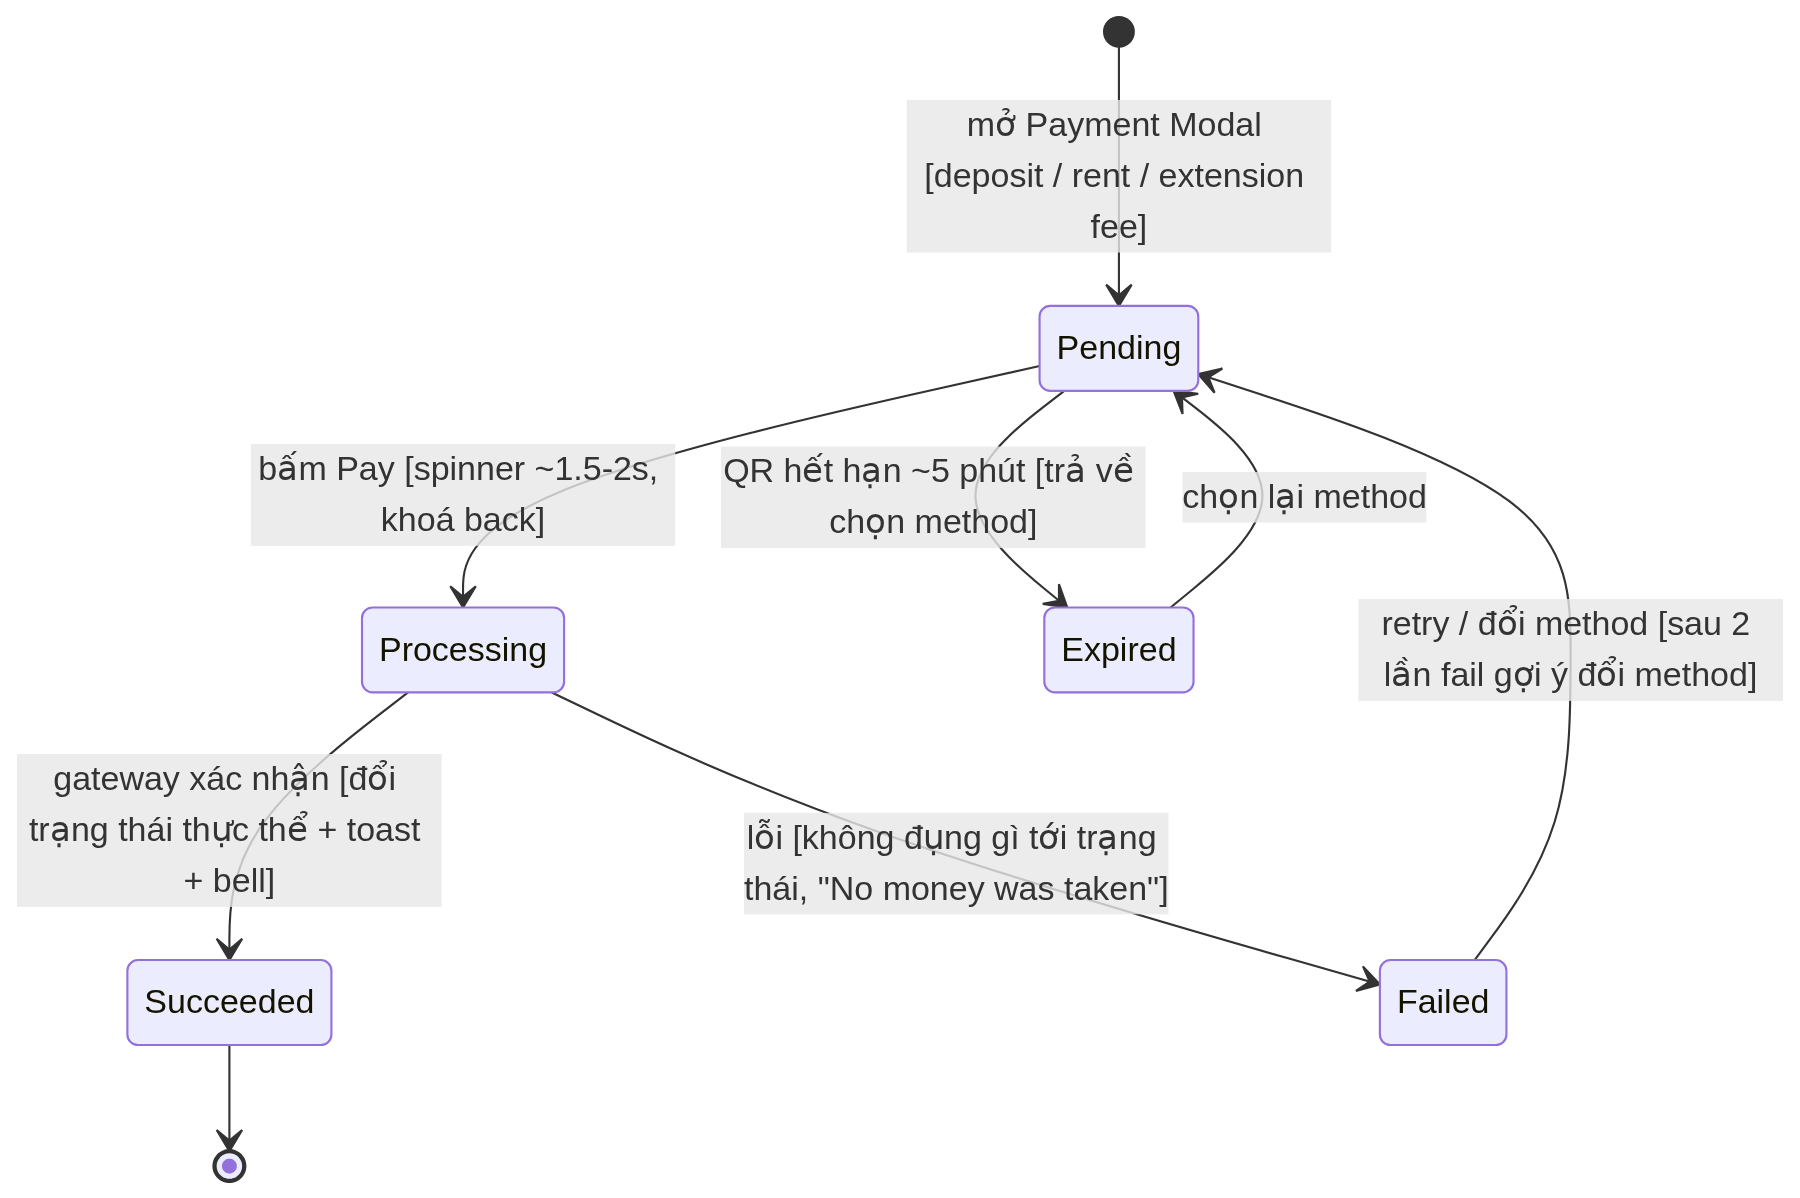
\includegraphics[width=\textwidth]{state-payment.png}
\caption{State chart Payment}
\label{fig:state-payment}
\end{figure}

%===========================================================
% PHỤ LỤC: MÃ MERMAID CHO CÁC SƠ ĐỒ
%===========================================================
\section{PHỤ LỤC: MÃ MERMAID CHO CÁC SƠ ĐỒ}

Toàn bộ mã nguồn Mermaid đã dùng để render 8 ảnh trong tài liệu (ERD + 7 state chart). Ảnh được render qua kroki.io / mermaid.ink ở độ rộng 1800px.

\subsection{Mermaid \#1 -- ERD (22 thực thể, 8 nhóm)}

\begin{mermaidbox}{Mermaid: ERD -- erd.mmd}
\begin{Verbatim}[fontsize=\small]
%% StorageHub - ERD (crow's foot) - 22 thuc the, 8 nhom
%% Nen tang: EXPERIENCE.md (ux-swp391-2026-09-11) + 7 flows swimlane + tinh nang hop dong CT-
erDiagram
    %% ── Nhom 1: Nguoi dung & co so ──
    ROLES ||--o{ USERS : "phan vai"
    FACILITIES ||--o{ ZONES : "co"
    ZONES ||--o{ UNITS : "chua"
    UNIT_TYPES ||--o{ UNITS : "phan loai"
    USERS ||--o{ STAFF_ASSIGNMENTS : "duoc gan"
    ZONES ||--o{ STAFF_ASSIGNMENTS : "phu trach"

    %% ── Nhom 2: Kho & chinh sach ──
    RENTAL_POLICIES ||--o{ POLICY_RULES : "dinh nghia"
    UNIT_TYPES ||--o{ POLICY_RULES : "ap dung cho"

    %% ── Nhom 3: Dat & thue ──
    USERS ||--o{ RESERVATIONS : "dat"
    UNITS ||--o{ RESERVATIONS : "duoc giu"
    RESERVATIONS ||--|| RENTALS : "kich hoat"
    USERS ||--o{ RENTALS : "thue"
    UNITS ||--o{ RENTALS : "cho thue"
    RENTALS ||--o{ EXTENSIONS : "gia han"
    RENTALS ||--o{ CHECKOUT_REQUESTS : "xin tra"

    %% ── Nhom 4: Hop dong ──
    RENTALS ||--o{ CONTRACTS : "mang"
    CONTRACTS ||--o{ CONTRACTS : "phu luc cua"
    RENTAL_POLICIES ||--o{ CONTRACTS : "khoa phien ban"

    %% ── Nhom 5: Tien ──
    USERS ||--o{ PAYMENTS : "thanh toan"
    RESERVATIONS ||--o{ PAYMENTS : "deposit 10%"
    RENTALS ||--o{ PAYMENTS : "rent 100%"
    EXTENSIONS ||--o| PAYMENTS : "phi gia han"
    SETTLEMENTS ||--o{ PAYMENTS : "damage / extra"

    %% ── Nhom 6: Tra kho & thanh ly ──
    RENTALS ||--o| SETTLEMENTS : "thanh ly"
    CONTRACTS ||--o{ SETTLEMENTS : "doi chieu"
    SETTLEMENTS ||--o{ INSPECTIONS : "kiem hang muc"

    %% ── Nhom 7: Ho tro ──
    USERS ||--o{ SUPPORT_TICKETS : "gui"
    UNITS ||--o{ SUPPORT_TICKETS : "lien quan"
    RENTALS ||--o{ SUPPORT_TICKETS : "thuoc phien thue"
    SUPPORT_TICKETS ||--o| ESCALATIONS : "duoc nang cap"

    %% ── Nhom 8: Van hanh & he thong ──
    USERS ||--o{ TASKS : "nhan viec"
    USERS ||--o{ NOTIFICATIONS : "nhan"
    USERS ||--o{ ACTIVITY_LOGS : "ghi audit"
    UNITS ||--o{ UNITS : "merge vao"

    ROLES {
        int RoleID PK
        varchar Name UK
        varchar Description
    }
    USERS {
        bigint UserID PK
        varchar FullName
        varchar Email UK
        varchar Phone
        varchar PasswordHash
        int RoleID FK
        tinyint Status
        datetime CreatedAt
    }
    FACILITIES {
        int FacilityID PK
        varchar Name
        varchar Address
        varchar Phone
        tinyint Status
    }
    ZONES {
        int ZoneID PK
        int FacilityID FK
        varchar Code
        int Floor
    }
    STAFF_ASSIGNMENTS {
        bigint AssignmentID PK
        bigint StaffID FK
        int ZoneID FK
        enum Shift
        date WorkDate
    }
    UNIT_TYPES {
        int TypeID PK
        varchar Name
        varchar Description
    }
    UNITS {
        bigint UnitID PK
        varchar Code UK
        int TypeID FK
        int ZoneID FK
        decimal SizeM2
        int Floor
        varchar AccessType
        enum Status
        bigint MergedIntoID FK
    }
    RENTAL_POLICIES {
        int PolicyID PK
        varchar Version UK
        date EffectiveDate
        tinyint Status
    }
    POLICY_RULES {
        bigint RuleID PK
        int PolicyID FK
        int TypeID FK
        enum RuleType
        enum SurchargeType
        decimal Value
        decimal Cap
    }
    RESERVATIONS {
        bigint ReservationID PK
        varchar Code UK
        bigint CustomerID FK
        bigint UnitID FK
        date StartDate
        date EndDate
        decimal DepositAmount
        enum Status
    }
    RENTALS {
        bigint RentalID PK
        varchar Code UK
        bigint ReservationID FK
        bigint CustomerID FK
        bigint UnitID FK
        date EndDate
        varchar AccessCode
        decimal DepositHeld
        enum Status
    }
    EXTENSIONS {
        bigint ExtensionID PK
        bigint RentalID FK
        date OldEndDate
        date NewEndDate
        decimal ExtensionFee
        enum Status
    }
    CHECKOUT_REQUESTS {
        bigint RequestID PK
        bigint RentalID FK
        date RequestedDate
        enum Status
    }
    CONTRACTS {
        bigint ContractID PK
        varchar Code UK
        bigint RentalID FK
        bigint ParentContractID FK
        int PolicyID FK
        enum Type
        text ContentSnapshot
        varchar SignedPhotoUrl
        date SignatureDueDate
        enum Status
    }
    PAYMENTS {
        bigint PaymentID PK
        varchar ReceiptCode UK
        bigint PayerID FK
        bigint ReservationID FK
        bigint RentalID FK
        bigint ExtensionID FK
        bigint SettlementID FK
        enum Purpose
        enum Method
        decimal Amount
        enum Status
    }
    SETTLEMENTS {
        bigint SettlementID PK
        bigint RentalID FK
        bigint ContractID FK
        bigint StaffID FK
        decimal DamageFee
        varchar DamageReason
        decimal RefundAmount
        varchar ReceiptCode UK
    }
    INSPECTIONS {
        bigint InspectionID PK
        bigint SettlementID FK
        enum Item
        enum Result
        varchar Note
    }
    SUPPORT_TICKETS {
        bigint TicketID PK
        varchar Code UK
        bigint CustomerID FK
        bigint UnitID FK
        bigint RentalID FK
        enum IncidentType
        enum Status
        bigint AssignedStaffID FK
    }
    ESCALATIONS {
        bigint EscalationID PK
        bigint TicketID FK
        bigint EscalatedByStaffID FK
        bigint ManagerID FK
        text Note
        enum Decision
    }
    TASKS {
        bigint TaskID PK
        enum Type
        varchar RefCode
        bigint AssignedStaffID FK
        date WorkDate
        enum Status
    }
    NOTIFICATIONS {
        bigint NotificationID PK
        bigint UserID FK
        varchar Type
        varchar Title
        varchar DeepLink
        tinyint IsRead
    }
    ACTIVITY_LOGS {
        bigint LogID PK
        bigint ActorID FK
        varchar EntityType
        bigint EntityID
        varchar Action
        varchar FromValue
        varchar ToValue
        varchar Reason
    }
\end{Verbatim}
\end{mermaidbox}

\subsection{Mermaid \#2 -- State chart: Unit}

\begin{mermaidbox}{Mermaid: State chart Unit}
\begin{Verbatim}[fontsize=\small]
%% StorageHub - State chart: vong doi Unit (kho)
stateDiagram-v2
    direction LR
    [*] --> Available : tao unit moi

    Available --> Reserved : deposit 10% thanh cong
    Reserved --> Rented : check-in hoan tat (hop dong da ky)
    Reserved --> Available : het han giu cho / huy dat

    Rented --> Preparing : checkout + settlement hoan tat
    Preparing --> Available : cleaning task xong
    Preparing --> Reserved : cleaning xong [co reservation ke tiep]

    Rented --> Maintenance : escalate muc severe
    Available --> Maintenance : manager set [bat buoc reason]
    Maintenance --> Preparing : sua chua xong
    Maintenance --> Retired : bo khoi ton kho

    Available --> Retired : retire [guard: khong rental/reservation]
    Reserved --> Retired : retire [guard: khong rental/reservation]

    note right of Available
        Buffer khong phai trang thai rieng:
        Available + ngay bat dau tre
        (turnover buffer) hien thi
        "Available soon" tren Browse.
    end note
    note right of Rented
        Merge 2 unit lien ke [guard:
        khong rental/reservation ca 2 phia]
        tao unit moi, unit cu ve Retired.
    end note
\end{Verbatim}
\end{mermaidbox}

\subsection{Mermaid \#3 -- State chart: Reservation}

\begin{mermaidbox}{Mermaid: State chart Reservation}
\begin{Verbatim}[fontsize=\small]
%% StorageHub - State chart: vong doi Reservation (BK-)
stateDiagram-v2
    [*] --> PendingPayment : KH dat unit (Booking Summary)

    PendingPayment --> Reserved : payment gateway xac nhan deposit
    PendingPayment --> PendingPayment : payment fail [retry / doi method]
    PendingPayment --> [*] : KH bo qua [khong giu unit]

    Reserved --> CheckedIn : tra 100% rent + ky hop dong (sinh Rental)
    Reserved --> Expired : qua han check-in [unit tra ve Available]
    Reserved --> Cancelled : huy dat [hoan deposit theo policy]

    CheckedIn --> [*]
\end{Verbatim}
\end{mermaidbox}

\subsection{Mermaid \#4 -- State chart: Rental}

\begin{mermaidbox}{Mermaid: State chart Rental}
\begin{Verbatim}[fontsize=\small]
%% StorageHub - State chart: vong doi Rental (RT-)
stateDiagram-v2
    [*] --> Active : check-in xong (cap access code)

    Active --> Active : gia han [fee da tra: EndDate dich ngay]
                       (sinh addendum cho ky)
    Active --> CheckoutRequested : KH gui checkout request

    CheckoutRequested --> Closed : settlement hoan tat
                                [refund = deposit - damage fee]
    Closed --> [*]

    note right of Active
        Gia han hieu luc ngay sau
        thanh toan - phu luc CT chi la
        paperwork, khong hold unit.
        Conflict guard: khong de
        reservation ke tiep
        ("Latest new checkout: Oct 18").
    end note
\end{Verbatim}
\end{mermaidbox}

\subsection{Mermaid \#5 -- State chart: Contract}

\begin{mermaidbox}{Mermaid: State chart Contract}
\begin{Verbatim}[fontsize=\small]
%% StorageHub - State chart: vong doi Contract (CT-)
stateDiagram-v2
    [*] --> Draft : auto-draft [ngay khi deposit thanh cong,
                                   khoa policy version]

    Draft --> Printed : staff in tai quay
    Printed --> Signed : KH ky + staff chup anh attach
    Signed --> Active : rental kich hoat (hop dong goc)
    Active --> Closed : settlement tham chieu so hop dong
    Active --> Superseded : addendum thay ngay ket thuc

    Draft --> AwaitingSignature : addendum gia han
                                        [auto-draft sau khi tra fee]
    AwaitingSignature --> Signed : ky tai quay [deadline 7 ngay,
                                                        bell reminder]
    AwaitingSignature --> AwaitingSignature : qua han
                                              [banner amber + nhac viec]

    Signed --> [*] : addendum da filed
    Closed --> [*]

    note right of Printed
        Printed chan cap access code
        den khi co anh ban ky.
        Hop dong khong ai sua duoc -
        chinh = draft lai.
    end note
\end{Verbatim}
\end{mermaidbox}

\subsection{Mermaid \#6 -- State chart: Support Ticket}

\begin{mermaidbox}{Mermaid: State chart Support Ticket}
\begin{Verbatim}[fontsize=\small]
%% StorageHub - State chart: vong doi Support Ticket (SR-)
stateDiagram-v2
    [*] --> Open : KH gui support request

    Open --> InProgress : route toi staff truc ca [theo unit + shift]
    InProgress --> Resolved : staff xu ly xong + note
    InProgress --> Escalated : staff escalate [bat buoc co note]

    Escalated --> Resolved : manager danh gia severe
                             [unit -> Maintenance + tai dinh vi KH]
    Escalated --> InProgress : manager tra ve staff [kem guidance]

    Resolved --> [*]

    note right of Escalated
        Ticket severe khong bi bo roi:
        quyet dinh ghi vao Activity Log,
        KH nhan notification tung buoc.
    end note
\end{Verbatim}
\end{mermaidbox}

\subsection{Mermaid \#7 -- State chart: Task}

\begin{mermaidbox}{Mermaid: State chart Task}
\begin{Verbatim}[fontsize=\small]
%% StorageHub - State chart: vong doi Task (kanban)
stateDiagram-v2
    [*] --> ToDo : he thong sinh task
                    [check-in / checkout / cleaning / support / contract]

    ToDo --> InProgress : staff keo tha hoac mo task
    InProgress --> Done : hoan tat buoc chot
                           [guard: payment / settlement / anh ban ky]
    Done --> InProgress : snap-back [thieu buoc chot] + toast chi ten buoc thieu

    Done --> [*]
\end{Verbatim}
\end{mermaidbox}

\subsection{Mermaid \#8 -- State chart: Payment}

\begin{mermaidbox}{Mermaid: State chart Payment}
\begin{Verbatim}[fontsize=\small]
%% StorageHub - State chart: vong doi Payment (mock gateway, 3 touchpoint)
stateDiagram-v2
    [*] --> Pending : mo Payment Modal [deposit / rent / extension fee]

    Pending --> Processing : bam Pay [spinner ~1.5-2s, khoa back]
    Processing --> Succeeded : gateway xac nhan
                                 [doi trang thai thuc the + toast + bell]
    Processing --> Failed : loi [khong dung gi toi trang thai,
                                  "No money was taken"]

    Failed --> Pending : retry / doi method [sau 2 lan fail goi y doi method]
    Pending --> Expired : QR het han ~5 phut [tra ve chon method]

    Succeeded --> [*]
    Expired --> Pending : chon lai method
\end{Verbatim}
\end{mermaidbox}

\end{document}
